% Provenance (never printed): see sources/outline_sources.md (Year 1: fault types and
% Anderson's theory; fold geometry and classification; foliation, schistosity and
% lineation; microstructures). Exercise and problem values in the Book 3 scratch calculator
% calc/ch17.py; the Varden Hills fold and fault from figdata/shared/region.py (read only).
% Fold, anticline, syncline and fold axis are owned by ch. 4; throw and heave by ch. 5;
% trend and plunge by ch. 6; the stresses and the Coulomb criterion by ch. 16. Shear zones
% and deformation mechanisms belong to the Year 3 volume (told here).
\chapter{Failles, plis et fabriques}\label{ch:b1:faults-folds-fabrics}

Une tranchée de route montre une face de roche polie comme du verre et rayée de fines
cannelures parallèles. De l'autre côté de la vallée, une falaise marine montre des bancs de grès et
de schiste pliés en zigzags aux côtés droits et aux angles vifs. Sur un toit
voisin, des ardoises se débitent en feuillets de quelques millimètres d'épaisseur, selon des plans qui
recoupent les couches de la boue dont elles sont faites. Chacun est un enregistrement de la
déformation de la roche, lu à une échelle différente~: les cannelures donnent la direction
dans laquelle deux blocs ont glissé l'un contre l'autre le long d'une faille~; les zigzags mesurent de combien
les bancs ont été raccourcis~; les plans de l'ardoise ont poussé en travers du grain de la roche
tandis qu'elle était comprimée. Ce chapitre donne la géométrie nécessaire pour mesurer ces trois
enregistrements, et la mécanique du chapitre précédent explique pourquoi les failles prennent les
\omterm{def:b1:geological-maps:attitude}{pendages} qu'elles ont.

\begin{recall}
L'\omterm{def:b1:geological-maps:attitude}{attitude} d'un plan est son \omterm{def:b1:geological-maps:attitude}{sens du pendage} et son \omterm{def:b1:geological-maps:attitude}{pendage}, notée par exemple
$080/12$~; sa direction s'en déduit par la règle de la main droite, le plan plongeant à
droite d'un observateur qui regarde le long de la direction (\cref{ch:b1:geological-maps}).
Un \omterm{def:b1:geological-maps:fold}{pli} est une courbure de couches autrefois planes~; un \omterm{def:b1:geological-maps:fold}{anticlinal} est convexe vers le haut avec
les roches les plus anciennes en son cœur, un \omterm{def:b1:geological-maps:fold}{synclinal} concave vers le haut~; l'\omterm{def:b1:geological-maps:fold}{axe du pli} est la
ligne le long de laquelle les couches se courbent le plus (\cref{ch:b1:geological-maps}). Le
\omterm{def:b1:cross-sections:throw}{rejet vertical} et le \omterm{def:b1:cross-sections:throw}{rejet horizontal} d'une faille sont les composantes verticale et horizontale de son
déplacement (\cref{ch:b1:cross-sections}). Une droite a une direction et un \omterm{def:b1:field-lab-methods-1:trend-plunge}{plongement},
et le vecteur unitaire vers le bas $(\cos p\sin t, \cos p\cos t, -\sin p)$
(\cref{ch:b1:field-lab-methods-1}). Une roche qui obéit au critère de Coulomb
se rompt sur des plans à $\ang{45} - \phi/2$ de $\sigma_1$, et les failles existantes
glissent selon la \omterm{prop:b1:stress-strain-rheology:byerlee}{loi de Byerlee} (\cref{ch:b1:stress-strain-rheology}). Un
\omterm{def:b1:rock-forming-minerals:mineral}{minéral} est en extinction entre \omterm{def:b1:field-lab-methods-1:microscope}{polariseurs croisés} quand ses directions de vibration
sont parallèles à celles des polariseurs (\cref{ch:b1:optical-mineralogy}). Les failles
ont été rencontrées au livre~1, année~7~; les \omterm{def:b1:faults-folds-fabrics:fault-types}{failles inverses}, les \omterm{def:b1:faults-folds-fabrics:fault-types}{chevauchements} et la \omterm{def:b1:faults-folds-fabrics:foliation}{foliation} au livre~2,
année~12. Le produit vectoriel de deux vecteurs est perpendiculaire aux deux
(mathématiques, première année).
\end{recall}

\section{Les failles~: géométrie et cinématique}\label{sec:b1:faults-folds-fabrics:faults}

Une faille est une surface à travers laquelle deux blocs de roche se sont déplacés l'un
contre l'autre. Pour décrire le mouvement il faut des noms pour les deux blocs et pour le
déplacement, et un moyen de mesurer sa direction dans le plan de la
faille.

\begin{definition}[Compartiment supérieur, compartiment inférieur, vecteur glissement, glissement net, pitch]\label{def:b1:faults-folds-fabrics:fault-elements}
Soit une faille localement plane et non verticale. Le \emph{compartiment
supérieur}\index{compartiment superieur@compartiment supérieur} (ou toit) est le bloc au-dessus d'elle, le
\emph{compartiment inférieur}\index{compartiment inferieur@compartiment inférieur} (ou mur) le bloc en dessous. Soit $A$ un point du
compartiment inférieur et $A'$ le point du compartiment supérieur qui était en contact avec lui
avant le mouvement. Le \emph{vecteur glissement}\index{vecteur glissement}
$\overrightarrow{AA'}$ est le déplacement du compartiment supérieur par rapport au
compartiment inférieur~; sa longueur est le \emph{glissement net}\index{glissement net}. Le
\emph{pitch}\index{pitch} $r$ du vecteur glissement est
l'angle, mesuré dans le plan de la faille, de la direction donnée par
la règle de la main droite au vecteur glissement, positif quand le vecteur glissement pointe vers le haut
du plan et négatif quand il pointe vers le bas~: $\ang{-180} < r \le \ang{180}$. C'est la
convention des sismologues, reprise pour les séismes au \cref{ch:b1:earthquake-source}~; de nombreux
géologues de terrain notent plutôt un angle entre 0 et \ang{180}, mesuré
dans le sens horaire à partir de la direction vue de dessus, et ajoutent le sens du mouvement en mots.
\end{definition}
% ledger: ar:rake, ws:rake, ws:fault-terms

Les deux noms viennent de l'exploitation minière~: un mineur travaillant un filon incliné se tenait sur le
mur et avait le toit au-dessus de la tête. Un déplacement vu dans une seule
coupe n'est pas, en général, le glissement~: un banc décalé sur une carte ou dans une
coupe montre une séparation, qui dépend de l'\omterm{def:b1:geological-maps:attitude}{attitude} du banc. Le glissement
demande deux points qui n'en faisaient qu'un, comme les deux moitiés d'une ligne coupée par
la faille, par exemple le bord d'un dyke contre un banc.

\begin{omfigure}
\begin{tikzpicture}[>={Stealth[length=5pt]}, font=\small]
% (a) the fault plane seen face-on; slip vector of length 3.6 cm at rake -35 deg
% (normal and sinistral): strike-slip component 3.6 cos 35 = 2.949, dip-slip 3.6 sin 35 = 2.065
\pgfmathsetmacro{\Ls}{3.6*cos(35)}\pgfmathsetmacro{\Ld}{3.6*sin(35)}
\begin{scope}
  \fill[omDef!15] (0,0) rectangle (6.2,3.4);
  \draw[omDef, line width=0.7pt] (0,0) rectangle (6.2,3.4);
  \draw[line width=1.2pt] (0,3.4) -- (6.2,3.4);
  \node[anchor=south, font=\scriptsize] at (3.1,3.4) {ligne de direction, là où la faille rencontre le sol};
  \draw[->, line width=0.6pt] (6.45,3.0) -- (6.45,2.0) node[midway, right, font=\scriptsize, align=left] {vers le bas\\ du pendage};
  \draw[->, line width=0.6pt] (0.3,0.35) -- (1.3,0.35) node[right, font=\scriptsize] {direction};
  \coordinate (A) at (1.2,2.55);
  \coordinate (B) at ($(A)+(\Ls,0)$);
  \coordinate (A2) at ($(A)+(\Ls,-\Ld)$);
  \draw[omProp, dashed, line width=0.7pt] (A) -- (B) node[midway, above, xshift=4mm, font=\scriptsize] {composante en direction};
  \draw[omProp, dashed, line width=0.7pt] (B) -- (A2) node[midway, right, font=\scriptsize, align=left] {composante\\ en pendage};
  \draw[->, line width=1.3pt, omThm] (A) -- (A2) node[midway, below left, font=\scriptsize, inner sep=1pt] {vecteur glissement};
  \draw[black] ($(A)+(0.9,0)$) arc[start angle=0, end angle=-35, radius=0.9];
  \node[font=\scriptsize] at ($(A)+(-17.5:1.15)$) {$r$};
  \fill (A) circle[radius=1.4pt] node[above left, inner sep=1.5pt] {$A$};
  \fill (A2) circle[radius=1.4pt] node[below right, inner sep=1.5pt] {$A'$};
  \node[font=\small\bfseries] at (3.1,-0.55) {(a) dans le plan de la faille};
\end{scope}
% (b) the vertical section through the dip line: dip 50 deg; dip-slip 2.065 -> throw 1.582, heave 1.327
\begin{scope}[xshift=9.4cm, yshift=0.2cm]
  \pgfmathsetmacro{\th}{\Ld*sin(50)}\pgfmathsetmacro{\he}{\Ld*cos(50)}
  \fill[omLithSand!40] (-1.2,0) -- (-1.2,3.2) -- (0,3.2) -- ({3.2/tan(50)},0) -- cycle;
  \fill[omLithSand!20] ({3.2/tan(50)},0) -- (0,3.2) -- (4.2,3.2) -- (4.2,0) -- cycle;
  \draw[line width=0.6pt] (-1.2,3.2) -- (4.2,3.2);
  \draw[omDef, line width=1.1pt] (0,3.2) -- ({3.2/tan(50)},0);
  \draw[black] (0.75,3.2) arc[start angle=0, end angle=-50, radius=0.75];
  \node[font=\scriptsize] at ($(0,3.2)+(-25:1.0)$) {$\delta$};
  \coordinate (P) at ({1.3*cos(50)},{3.2-1.3*sin(50)});
  \coordinate (Q) at ($(P)+({\Ld*cos(50)},{-\Ld*sin(50)})$);
  \coordinate (R) at ($(P)+(\he,0)$);
  \draw[->, omProp, line width=1.1pt] (P) -- (Q);
  \draw[black!80, densely dotted, line width=0.7pt] (P) -- (R) node[midway, above, xshift=5mm, font=\scriptsize] {rejet horizontal};
  \draw[black!80, densely dotted, line width=0.7pt] (R) -- (Q) node[midway, right, font=\scriptsize] {rejet vertical};
  \node[font=\scriptsize, omProp, anchor=east] at ($(P)!0.55!(Q)+(-0.08,0)$) {jeu en pendage};
  \node[font=\small, align=center] at (3.4,0.55) {compartiment\\supérieur};
  \node[font=\small, align=center] at (-0.05,0.9) {compartiment\\inférieur};
  \node[font=\small\bfseries] at (1.5,-0.75) {(b) dans le plan vertical du pendage};
\end{scope}
\end{tikzpicture}
\par\smallskip{\small Les éléments d'une faille, dessinés à l'échelle pour une faille
de \omterm{def:b1:geological-maps:attitude}{pendage} $\delta = \ang{50}$ et un \omterm{def:b1:faults-folds-fabrics:fault-elements}{vecteur glissement} de \omterm{def:b1:faults-folds-fabrics:fault-elements}{pitch} $r = \ang{-35}$. (a) Le
plan de faille vu de face~: le \omterm{def:b1:faults-folds-fabrics:fault-elements}{vecteur glissement} $\overrightarrow{AA'}$ se décompose en une
composante selon la direction et une selon le \omterm{def:b1:geological-maps:attitude}{pendage}. (b) La coupe verticale
perpendiculaire à la direction~: la composante en \omterm{def:b1:geological-maps:attitude}{pendage} se décompose en \omterm{def:b1:cross-sections:throw}{rejet vertical}
et \omterm{def:b1:cross-sections:throw}{rejet horizontal}.}
\label{fig:b1:faults-folds-fabrics:elements}
\end{omfigure}

\begin{proposition}[Composantes du glissement]\label{prop:b1:faults-folds-fabrics:slip-components}
Soit une faille de \omterm{def:b1:geological-maps:attitude}{sens du pendage} $\alpha$ et de \omterm{def:b1:geological-maps:attitude}{pendage} $\delta$, et un \omterm{def:b1:faults-folds-fabrics:fault-elements}{vecteur glissement} de
longueur $L$ et de \omterm{def:b1:faults-folds-fabrics:fault-elements}{pitch} $r$. Avec des composantes est, nord et haut, soit
$\mathbf s = (\sin(\alpha-\ang{90}), \cos(\alpha-\ang{90}), 0)$ le vecteur unitaire
selon la direction et $\mathbf u = (-\cos\delta\sin\alpha,
-\cos\delta\cos\alpha, \sin\delta)$ le vecteur unitaire vers le haut du \omterm{def:b1:geological-maps:attitude}{pendage}. Alors
\[
  \overrightarrow{AA'} = L\,(\cos r\,\mathbf s + \sin r\,\mathbf u),
\]
sa composante en direction est $L\cos r$ et sa composante en \omterm{def:b1:geological-maps:attitude}{pendage} $L\sin r$~;
le \omterm{def:b1:cross-sections:throw}{rejet vertical} est $L\,|\sin r|\sin\delta$, le \omterm{def:b1:cross-sections:throw}{rejet horizontal} $L\,|\sin r|\cos\delta$, et
le \omterm{def:b1:faults-folds-fabrics:fault-elements}{vecteur glissement} plonge de $p$ avec $\sin p = |\sin r|\sin\delta$.
\end{proposition}

\begin{proof}
Le vecteur $\mathbf s$ est horizontal et pointe selon la direction~; $\mathbf u$
est l'opposé du vecteur unitaire vers le bas de la ligne de plus grande pente, qui a pour direction
$\alpha$ et pour \omterm{def:b1:field-lab-methods-1:trend-plunge}{plongement} $\delta$ (\cref{ch:b1:field-lab-methods-1}). Les deux sont dans
le plan de faille, et $\mathbf s\cdot\mathbf u = -\cos\delta(\sin(\alpha -
\ang{90})\sin\alpha + \cos(\alpha - \ang{90})\cos\alpha) = -\cos\delta\cos\ang{90} = 0$,
donc ils forment une base orthonormée du plan. Un vecteur du plan de
longueur $L$ à l'angle $r$ de $\mathbf s$, compté vers $\mathbf u$, est
$L(\cos r\,\mathbf s + \sin r\,\mathbf u)$. Sa composante verticale est
$L\sin r\sin\delta$, dont la valeur est le \omterm{def:b1:cross-sections:throw}{rejet vertical}~; sa partie horizontale en travers de la
direction est $L\sin r$ fois la partie horizontale de $\mathbf u$, de longueur
$\cos\delta$, qui est le \omterm{def:b1:cross-sections:throw}{rejet horizontal}~; et le sinus de son \omterm{def:b1:field-lab-methods-1:trend-plunge}{plongement} est sa composante
verticale divisée par $L$.
\end{proof}

Pour une faille à glissement en \omterm{def:b1:geological-maps:attitude}{pendage}, $|\sin r| = 1$ et le \omterm{def:b1:cross-sections:throw}{rejet horizontal} est le \omterm{def:b1:cross-sections:throw}{rejet vertical} divisé par
$\tan\delta$, comme au \cref{ch:b1:cross-sections}. Le \omterm{def:b1:faults-folds-fabrics:fault-elements}{pitch} classe les failles
en familles.

\begin{definition}[Failles normales, inverses, chevauchements, décrochantes et obliques]\label{def:b1:faults-folds-fabrics:fault-types}
Une faille dont le \omterm{def:b1:faults-folds-fabrics:fault-elements}{vecteur glissement} est le long de la ligne de plus grande pente ($r = \pm\ang{90}$) est une
faille à glissement en \omterm{def:b1:geological-maps:attitude}{pendage}~: une \emph{faille normale}\index{faille normale} quand le \omterm{def:b1:faults-folds-fabrics:fault-elements}{compartiment supérieur}
s'est abaissé ($r = \ang{-90}$), une \emph{faille inverse}\index{faille inverse} quand il s'est élevé
($r = \ang{90}$). Un \emph{chevauchement}\index{chevauchement} est une faille inverse de \omterm{def:b1:geological-maps:attitude}{pendage} \ang{45} ou moins.
Une faille dont le glissement est parallèle à sa direction ($r = 0$ ou \ang{180}) est une
\emph{faille décrochante}\index{faille decrochante@faille décrochante}~; de telles failles sont en général
presque verticales. Une faille décrochante est \emph{dextre}\index{dextre}
quand un observateur placé d'un côté voit l'autre côté
déplacé vers la droite, \emph{senestre}\index{senestre} quand c'est vers
la gauche. Une faille dont le glissement a à la fois une composante en direction et une composante en \omterm{def:b1:geological-maps:attitude}{pendage}
est une \emph{faille oblique}\index{faille oblique}~; en pratique une
faille est nommée d'après sa composante la plus grande, de sorte qu'un \omterm{def:b1:faults-folds-fabrics:fault-elements}{pitch} proche de \ang{-90} est
dit normal.
\end{definition}
% ledger: usgs:fault-types, ws:fault-terms, ar:rake

\begin{proposition}[Le sens d'une faille décrochante]\label{prop:b1:faults-folds-fabrics:sense}
Le sens d'une \omterm{def:b1:faults-folds-fabrics:fault-types}{faille décrochante} ne dépend pas du côté où se
tient l'observateur. Un \omterm{def:b1:faults-folds-fabrics:fault-elements}{pitch} proche de $0$ est \omterm{def:b1:faults-folds-fabrics:fault-types}{senestre}, un \omterm{def:b1:faults-folds-fabrics:fault-elements}{pitch} proche de \ang{180} \omterm{def:b1:faults-folds-fabrics:fault-types}{dextre}.
\end{proposition}

\begin{proof}
Si un observateur sur le bloc 1 voit le bloc 2 se déplacer de $\mathbf v$, un observateur sur
le bloc 2 voit le bloc 1 se déplacer de $-\mathbf v$. En se retournant pour faire face au bloc 1, le
second observateur a échangé la gauche et la droite. Les deux changements s'annulent~: les deux
voient l'autre côté aller dans le même sens, vers la droite ou vers la gauche. Pour la
seconde partie, tenons-nous sur le \omterm{def:b1:faults-folds-fabrics:fault-elements}{compartiment inférieur} face au \omterm{def:b1:faults-folds-fabrics:fault-elements}{compartiment supérieur}~: on regarde alors
vers le bas du \omterm{def:b1:geological-maps:attitude}{pendage}, et comme le plan plonge à droite de sa direction,
la direction pointe à notre gauche. Un \omterm{def:b1:faults-folds-fabrics:fault-elements}{pitch} de $0$ déplace le \omterm{def:b1:faults-folds-fabrics:fault-elements}{compartiment supérieur}
le long de la direction, vers la gauche~; un \omterm{def:b1:faults-folds-fabrics:fault-elements}{pitch} de \ang{180} le déplace vers la droite.
\end{proof}

Une surface de faille est souvent elle-même un enregistrement du mouvement~: les rayures et les
fibres qu'elle porte sont selon le glissement. Autour de la surface, une zone de faille peut être remplie
de roche brisée par le mouvement.

\begin{definition}[Miroir de faille, stries, roches de faille]\label{def:b1:faults-folds-fabrics:fault-rocks}
Les \emph{stries}\index{stries} sont des rayures ou des fibres sur une surface de
faille, parallèles au glissement~; un \emph{miroir de faille}\index{miroir de faille} est une
surface de faille qui les porte, souvent lissée par le glissement. Une \emph{roche
de faille}\index{roche de faille} est une roche faite par le mouvement sur une faille. Une
\emph{brèche de faille}\index{breche de faille@brèche de faille} est faite de fragments anguleux des
parois de la faille, tournés et déplacés, de blocs énormes jusqu'à
environ \qty{2}{mm}~; une \emph{cataclasite}\index{cataclasite} est faite de
fragments de la taille du sable ou plus petits~; ni l'une ni l'autre n'a de fabrique, les fragments étant
au hasard. Une \emph{gouge de faille}\index{gouge de faille} est une roche de faille riche en
argile, très tendre à l'\omterm{def:b1:geological-maps:geological-map}{affleurement}. Une \emph{mylonite}\index{mylonite} est une
roche à grain fin, fortement foliée, faite dans une zone de cisaillement par cisaillement ductile,
les grains réduits par recristallisation plutôt que par broyage.
\end{definition}
% ledger: ws:fault-terms, ws:fault-rocks

Les \omterm{def:b1:faults-folds-fabrics:fault-rocks}{roches de faille} sont une jauge de profondeur, et elles suivent l'\omterm{def:b1:stress-strain-rheology:strength-envelope}{enveloppe de résistance} du
\cref{ch:b1:stress-strain-rheology}. La gouge, la brèche et la \omterm{def:b1:faults-folds-fabrics:fault-rocks}{cataclasite}, avec
leur fabrique aléatoire, sont faites par glissement frictionnel et fracture dans la
\omterm{def:b1:layered-earth:layers}{croûte} cassante~; les \omterm{def:b1:faults-folds-fabrics:fault-rocks}{mylonites} sont faites sous la \omterm{def:b1:stress-strain-rheology:strength-envelope}{transition cassant--ductile}, où
la faille se prolonge vers le bas comme une bande de cisaillement ductile. Pour un
\omterm{def:b1:heat-budget:geotherm}{géotherme} normal et assez d'eau, la transition entre les deux se situe à
\qtyrange{10}{15}{km}, près des \qty{13.7}{km} de l'enveloppe du
chapitre précédent, et la faille y est la plus résistante. À travers une grande faille
remontée de la profondeur, le même ordre se retrouve côte à côte~: des zones de gouge près
de la surface, puis la \omterm{def:b1:faults-folds-fabrics:fault-rocks}{cataclasite}, puis la \omterm{def:b1:faults-folds-fabrics:fault-rocks}{mylonite}.
Le nom de \omterm{def:b1:faults-folds-fabrics:fault-rocks}{mylonite}, du mot grec pour moudre la farine, enregistre une erreur~:
on la croyait de la roche broyée. Le volume de troisième année étudie ces zones de cisaillement
profondes et les mécanismes qui font les \omterm{def:b1:faults-folds-fabrics:fault-rocks}{mylonites}.
% ledger: sibson:fault-rocks, sibson:alpine-fault, ws:fault-rocks

\begin{omfigure}
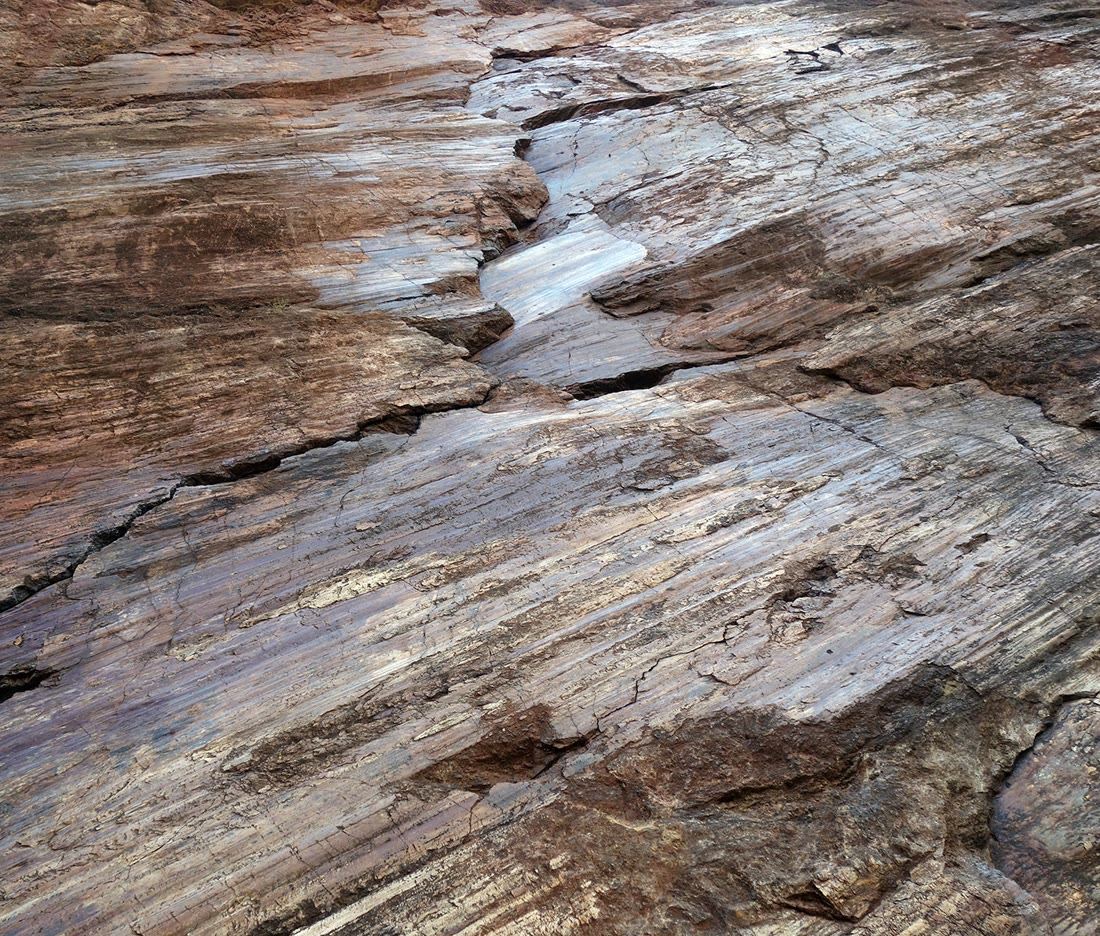
\includegraphics[height=5.2cm]{images/book3/b1-slickenside.jpg}\hfill
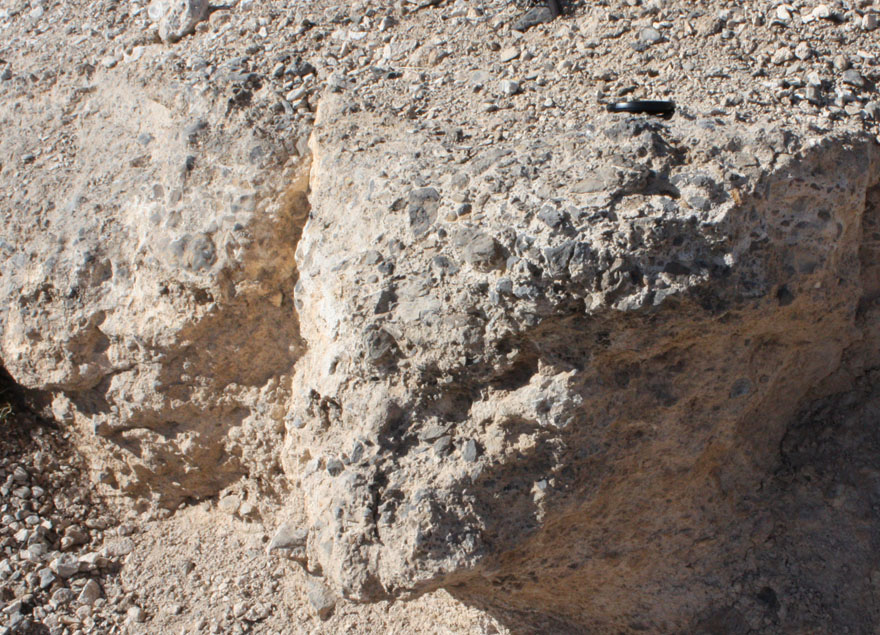
\includegraphics[height=5.2cm]{images/book3/b1-fault-breccia.jpg}
\par\smallskip{\small À gauche~: un \omterm{def:b1:faults-folds-fabrics:fault-rocks}{miroir de faille} sur une surface de faille dans du chert, environ
\qtyproduct{3 x 3}{m} d'une surface haute de \qty{10}{m}, Corona Heights, San
Francisco~; la face polie est striée selon le glissement. Photographie~:
Dextersinister, CC~BY-SA~4.0. À droite~: \omterm{def:b1:faults-folds-fabrics:fault-rocks}{brèche de faille} du \omterm{def:b1:faults-folds-fabrics:fault-types}{chevauchement} de Keystone, Red
Rock Canyon, Nevada~: fragments anguleux de roche carbonatée grise dans une
matrice plus pâle~; le cache d'objectif en haut à droite fait \qty{5.8}{cm} de large. Photographie~:
Jstuby, domaine public. Les deux proviennent de Wikimedia Commons.}
\label{fig:b1:faults-folds-fabrics:fault-surfaces}
\end{omfigure}
% ledger: commons:slickenside, commons:breccia

\begin{method}[Mesurer le glissement sur une faille]\label{met:b1:faults-folds-fabrics:slip}
\begin{enumerate}
  \item Mesurer l'\omterm{def:b1:geological-maps:attitude}{attitude} $\alpha/\delta$ de la surface de faille et écrire sa
        direction, $\alpha - \ang{90}$.
  \item Mesurer les \omterm{def:b1:faults-folds-fabrics:fault-rocks}{stries}~: leur \omterm{def:b1:faults-folds-fabrics:fault-elements}{pitch} sur la faille, ou leur direction et leur
        \omterm{def:b1:field-lab-methods-1:trend-plunge}{plongement}~; pour un \omterm{def:b1:faults-folds-fabrics:fault-elements}{pitch} $r$, $\sin p = |\sin r|\sin\delta$.
  \item Trouver dans quel sens le \omterm{def:b1:faults-folds-fabrics:fault-elements}{compartiment supérieur} s'est déplacé, à partir de repères décalés de part et d'autre de la
        faille, et donner son signe au \omterm{def:b1:faults-folds-fabrics:fault-elements}{pitch}~: négatif si le \omterm{def:b1:faults-folds-fabrics:fault-elements}{compartiment supérieur} est
        descendu.
  \item Trouver le \omterm{def:b1:faults-folds-fabrics:fault-elements}{glissement net} $L$ à partir de deux points qui n'en faisaient qu'un~; si seul le
        \omterm{def:b1:cross-sections:throw}{rejet vertical} $h$ d'un repère horizontal est connu, $L = h/(|\sin r|\sin\delta)$.
  \item Calculer les composantes avec
        la \cref{prop:b1:faults-folds-fabrics:slip-components} et nommer la faille
        avec la \cref{def:b1:faults-folds-fabrics:fault-types}.
\end{enumerate}
\end{method}

\begin{inthefield}[Mesurer une surface de faille]
Un géologue qui trouve une surface de faille sur un \omterm{def:b1:geological-maps:geological-map}{affleurement} la mesure comme n'importe quel autre
plan, avec une boussole-clinomètre posée sur la surface, puis mesure les
\omterm{def:b1:faults-folds-fabrics:fault-rocks}{stries} qui s'y trouvent, soit comme un \omterm{def:b1:faults-folds-fabrics:fault-elements}{pitch}, avec un rapporteur posé sur le plan, soit
comme une direction et un \omterm{def:b1:field-lab-methods-1:trend-plunge}{plongement}. Les deux se vérifient l'un l'autre avec la
formule de l'étape~2 de la méthode. Le sens du mouvement est la partie difficile. De petites
marches sur un \omterm{def:b1:faults-folds-fabrics:fault-rocks}{miroir de faille}, et des fibres de quartz ou de calcite qui ont poussé tandis que les
blocs s'écartaient, peuvent montrer dans quel sens est allé le bloc manquant, mais certaines marches
pointent dans le mauvais sens, si bien que le sens n'est cru que s'il s'accorde avec le
décalage d'un banc repère ou d'un filon. Les \omterm{def:b1:faults-folds-fabrics:fault-rocks}{roches de faille} sont décrites et échantillonnées, et une
zone de faille trop large pour être mesurée en un seul lieu est cartographiée comme une bande. Chaque faille est
consignée à une station numérotée du carnet, avec son \omterm{def:b1:geological-maps:attitude}{attitude}, ses
\omterm{def:b1:faults-folds-fabrics:fault-rocks}{stries}, le sens du mouvement et le degré de certitude du géologue.
\end{inthefield}

\section{La théorie d'Anderson de la fracturation}\label{sec:b1:faults-folds-fabrics:anderson}

Pourquoi la plupart des \omterm{def:b1:faults-folds-fabrics:fault-types}{failles normales} sont-elles raides et la plupart des \omterm{def:b1:faults-folds-fabrics:fault-types}{chevauchements} doux~? En 1905 le
géologue écossais Ernest Masson Anderson répondit par deux remarques~: la surface de la
Terre fixe les directions des \omterm{def:b1:stress-strain-rheology:principal}{contraintes principales}, et le critère de Coulomb
fixe alors l'angle des failles.
% ledger: ws:anderson, anderson:1905

\begin{proposition}[Une surface libre fait un plan principal]\label{prop:b1:faults-folds-fabrics:free-surface}
À la surface de la Terre, là où elle est horizontale, une contrainte principale est
verticale et les deux autres sont horizontales.
\end{proposition}

\begin{proof}
L'air ne presse sur le sol que par sa pression, normale à la surface~:
il n'exerce aucune contrainte de cisaillement. La contrainte sur le plan horizontal en surface
est donc normale à lui. En trois dimensions, la contrainte sur un plan de normale
unitaire $\mathbf n$ est le vecteur $\boldsymbol\sigma\mathbf n$ (livres de physique,
troisième année)~; si elle n'a pas de partie de cisaillement, elle est parallèle à $\mathbf n$, de sorte que
$\boldsymbol\sigma\mathbf n = \lambda\mathbf n$ et $\mathbf n$ est un
vecteur propre de la matrice symétrique $\boldsymbol\sigma$~: une direction
principale (\cref{def:b1:stress-strain-rheology:principal}). La verticale est
donc une direction principale, et les deux autres, perpendiculaires à elle, sont
horizontales.
\end{proof}

Anderson supposa que les \omterm{def:b1:stress-strain-rheology:principal}{contraintes principales} gardent ces directions jusqu'aux
profondeurs où se forment les failles. L'hypothèse tient bien sous une surface en pente
douce et dans des roches sans fortes faiblesses anciennes~; elle échoue près d'un
relief raide et là où d'anciennes failles ou couches guident les nouvelles. Avec elle, trois cas seulement
sont possibles, selon celle de $\sigma_1$, $\sigma_2$ et
$\sigma_3$ qui est verticale.

\begin{theorem}[La théorie d'Anderson de la fracturation]\label{thm:b1:faults-folds-fabrics:anderson}
Soit une contrainte principale verticale et que la roche se rompe selon le critère de
Coulomb, avec l'\omterm{def:b1:stress-strain-rheology:coulomb}{angle de frottement interne} $\phi$. De nouvelles failles se forment sur des
plans qui contiennent la direction de $\sigma_2$ et font l'angle
$\ang{45} - \phi/2$ avec $\sigma_1$, et elles glissent perpendiculairement à $\sigma_2$,
raccourcissant la roche selon $\sigma_1$. D'où
\begin{enumerate}[label=(\alph*)]
  \item si $\sigma_1$ est verticale, des \omterm{def:b1:faults-folds-fabrics:fault-types}{failles normales} se forment, de direction selon
        $\sigma_2$ et de \omterm{def:b1:geological-maps:attitude}{pendage} $\ang{45} + \phi/2$~;
  \item si $\sigma_3$ est verticale, des \omterm{def:b1:faults-folds-fabrics:fault-types}{chevauchements} se forment, de direction selon
        $\sigma_2$ et de \omterm{def:b1:geological-maps:attitude}{pendage} $\ang{45} - \phi/2$~;
  \item si $\sigma_2$ est verticale, des \omterm{def:b1:faults-folds-fabrics:fault-types}{failles décrochantes} verticales se forment, de direction
        à $\ang{45} - \phi/2$ de part et d'autre de $\sigma_1$.
\end{enumerate}
Avec $\phi = \ang{30}$, les \omterm{def:b1:geological-maps:attitude}{pendages} sont \ang{60}, \ang{30} et \ang{90}.
\end{theorem}
\index{theorie d'Anderson de la fracturation@théorie d'Anderson de la fracturation}

\begin{proof}
Sur un plan qui contient la direction de $\sigma_2$, la normale est dans le
plan de $\sigma_1$ et de $\sigma_3$, et la contrainte sur le plan est celle du
problème en deux dimensions du \cref{ch:b1:stress-strain-rheology}~: son point
se trouve sur le cercle de Mohr de $\sigma_1$ et de $\sigma_3$, et sa partie de cisaillement est
dans le plan de $\sigma_1$ et de $\sigma_3$, perpendiculaire à $\sigma_2$. Sur tout
autre plan, le point $(\sigma_n, \tau)$ est à l'intérieur de ce cercle, qui est
le plus grand des trois cercles de Mohr d'un état de contrainte tridimensionnel
(admis d'après la théorie tridimensionnelle). À mesure que les contraintes croissent, la droite
de Coulomb est donc d'abord touchée par des plans contenant $\sigma_2$, et parmi
eux, d'après le \cref{thm:b1:stress-strain-rheology:failure-angle}, par ceux à
$\ang{45} - \phi/2$ de $\sigma_1$. Le glissement sur un tel plan, perpendiculaire à
$\sigma_2$, rapproche les deux blocs selon la direction de plus forte
compression et les éloigne selon la plus faible, comme il le faut pour relâcher la
contrainte. Dans le cas (a) le plan fait l'angle $\ang{45} - \phi/2$ avec la
verticale, donc il plonge de $\ang{45} + \phi/2$~; il est de direction selon l'horizontale
$\sigma_2$~; le glissement est dans le plan vertical du \omterm{def:b1:geological-maps:attitude}{pendage}, et le bloc au-dessus
descend, allongeant la roche horizontalement~: une \omterm{def:b1:faults-folds-fabrics:fault-types}{faille normale}. Dans le cas (b) le
plan fait $\ang{45} - \phi/2 < \ang{45}$ avec l'horizontale $\sigma_1$, et
le glissement raccourcit la roche horizontalement, poussant le \omterm{def:b1:faults-folds-fabrics:fault-elements}{compartiment supérieur} vers le haut~: un
\omterm{def:b1:faults-folds-fabrics:fault-types}{chevauchement}. Dans le cas (c) les plans contiennent la verticale, donc ils sont
verticaux~; le glissement est horizontal, perpendiculaire à $\sigma_2$~: des \omterm{def:b1:faults-folds-fabrics:fault-types}{failles
décrochantes}, à $\ang{45} - \phi/2$ de part et d'autre de l'horizontale $\sigma_1$.
\end{proof}

Dans chaque régime deux familles de failles sont possibles, symétriques autour de $\sigma_1$~:
des failles conjuguées, se rencontrant à $\ang{90} - \phi$, environ \ang{60}, avec
$\sigma_1$ dans l'angle aigu entre elles. Inversement, une paire de failles conjuguées
mesurée sur le terrain donne les directions des contraintes qui les ont faites~:
$\sigma_1$ bissecte leur angle aigu, $\sigma_2$ est leur ligne
d'intersection.

\begin{omfigure}
\begin{tikzpicture}[x={(1cm,0cm)}, y={(0.42cm,0.30cm)}, z={(0cm,1cm)},
  >={Stealth[length=5pt]}, font=\small, scale=0.86,
  face/.style={draw=black, line width=0.5pt, line join=round},
  sone/.style={->, line width=1.6pt, omThm},
  sthree/.style={->, line width=0.8pt, omDef}]
% exact geometry: the fault plane is X = xf(Z); slip is along the dip; throw t
% (a) normal fault: dip 60, xf(Z) = 1.3 + (1.6 - Z)/tan 60, throw 0.45
\begin{scope}
  \def\W{3.2}\def\D{1.6}\def\H{1.6}
  \pgfmathsetmacro{\c}{1/tan(60)}
  \pgfmathsetmacro{\xa}{1.3+1.6*\c}       % xf(0)
  \pgfmathsetmacro{\xb}{1.3+0.45*\c}      % xf(H - t)
  \pgfmathsetmacro{\mfa}{1.3+(1.6-0.55)*\c}\pgfmathsetmacro{\mfb}{1.3+(1.6-0.85)*\c}
  \pgfmathsetmacro{\mha}{1.3+(1.6-0.10)*\c}\pgfmathsetmacro{\mhb}{1.3+(1.6-0.40)*\c}
  % footwall
  \fill[omLithSand!55] (0,0,0) -- (\xa,0,0) -- (1.3,0,\H) -- (0,0,\H) -- cycle;
  \fill[omProp!40] (0,0,0.55) -- (\mfa,0,0.55) -- (\mfb,0,0.85) -- (0,0,0.85) -- cycle;
  \draw[face] (0,0,0) -- (\xa,0,0) -- (1.3,0,\H) -- (0,0,\H) -- cycle;
  \draw[face, fill=omLithSand!35] (0,0,\H) -- (1.3,0,\H) -- (1.3,\D,\H) -- (0,\D,\H) -- cycle;
  \draw[face, fill=black!12] (1.3,0,\H) -- (\xb,0,1.15) -- (\xb,\D,1.15) -- (1.3,\D,\H) -- cycle;
  % hanging wall
  \fill[omLithSand!55] (\xa,0,0) -- (\W,0,0) -- (\W,0,1.15) -- (\xb,0,1.15) -- cycle;
  \fill[omProp!40] (\mha,0,0.10) -- (\W,0,0.10) -- (\W,0,0.40) -- (\mhb,0,0.40) -- cycle;
  \draw[face] (\xa,0,0) -- (\W,0,0) -- (\W,0,1.15) -- (\xb,0,1.15) -- cycle;
  \draw[face, fill=omLithSand!35] (\xb,0,1.15) -- (\W,0,1.15) -- (\W,\D,1.15) -- (\xb,\D,1.15) -- cycle;
  \fill[omLithSand!45] (\W,0,0) -- (\W,\D,0) -- (\W,\D,1.15) -- (\W,0,1.15) -- cycle;
  \fill[omProp!30] (\W,0,0.10) -- (\W,\D,0.10) -- (\W,\D,0.40) -- (\W,0,0.40) -- cycle;
  \draw[face] (\W,0,0) -- (\W,\D,0) -- (\W,\D,1.15) -- (\W,0,1.15) -- cycle;
  % slip arrow on the front face
  \draw[->, line width=0.9pt] (1.45,0,1.05) -- ++({0.35*cos(60)},0,{-0.35*sin(60)});
  % stresses: sigma1 vertical, sigma3 horizontal across the strike
  \draw[sone] (1.6,0.8,3.05) -- (1.6,0.8,2.1) node[pos=0, left] {$\sigma_1$};
  \draw[sone] (1.6,0.8,-1.1) -- (1.6,0.8,-0.15);
  \draw[sthree] (-0.85,0.8,0.8) -- (-0.15,0.8,0.8) node[pos=0, above] {$\sigma_3$};
  \draw[sthree] (4.05,0.8,0.6) -- (3.35,0.8,0.6);
  \node[font=\small\bfseries] at (1.9,0,-1.55) {(a) faille normale};
\end{scope}
% (b) thrust fault: dip 30, xf(Z) = 3.0 - Z/tan 30, throw 0.35, heave 0.606
\begin{scope}[xshift=6.0cm]
  \def\D{1.6}\def\H{1.3}
  \pgfmathsetmacro{\c}{1/tan(30)}
  \pgfmathsetmacro{\Wp}{4.0-0.35*\c}       % right face of the hanging wall
  \pgfmathsetmacro{\xt}{3.0-1.3*\c}        % footwall top edge
  \pgfmathsetmacro{\xh}{3.0-1.65*\c}       % hanging-wall top edge
  \pgfmathsetmacro{\mfa}{3.0-0.50*\c}\pgfmathsetmacro{\mfb}{3.0-0.75*\c}
  \pgfmathsetmacro{\mha}{3.0-0.85*\c}\pgfmathsetmacro{\mhb}{3.0-1.10*\c}
  % footwall
  \fill[omLithSand!55] (0,0,0) -- (3.0,0,0) -- (\xt,0,\H) -- (0,0,\H) -- cycle;
  \fill[omProp!40] (0,0,0.50) -- (\mfa,0,0.50) -- (\mfb,0,0.75) -- (0,0,0.75) -- cycle;
  \draw[face] (0,0,0) -- (3.0,0,0) -- (\xt,0,\H) -- (0,0,\H) -- cycle;
  \draw[face, fill=omLithSand!35] (0,0,\H) -- (\xt,0,\H) -- (\xt,\D,\H) -- (0,\D,\H) -- cycle;
  % hanging wall
  \fill[omLithSand!55] (3.0,0,0) -- (\Wp,0,0) -- (\Wp,0,1.65) -- (\xh,0,1.65) -- cycle;
  \fill[omProp!40] (\mha,0,0.85) -- (\Wp,0,0.85) -- (\Wp,0,1.10) -- (\mhb,0,1.10) -- cycle;
  \draw[face] (3.0,0,0) -- (\Wp,0,0) -- (\Wp,0,1.65) -- (\xh,0,1.65) -- cycle;
  \draw[face, fill=omLithSand!35] (\xh,0,1.65) -- (\Wp,0,1.65) -- (\Wp,\D,1.65) -- (\xh,\D,1.65) -- cycle;
  \fill[omLithSand!45] (\Wp,0,0) -- (\Wp,\D,0) -- (\Wp,\D,1.65) -- (\Wp,0,1.65) -- cycle;
  \fill[omProp!30] (\Wp,0,0.85) -- (\Wp,\D,0.85) -- (\Wp,\D,1.10) -- (\Wp,0,1.10) -- cycle;
  \draw[face] (\Wp,0,0) -- (\Wp,\D,0) -- (\Wp,\D,1.65) -- (\Wp,0,1.65) -- cycle;
  \draw[->, line width=0.9pt] (2.25,0,0.62) -- ++({-0.42*cos(30)},0,{0.42*sin(30)});
  % stresses: sigma1 horizontal across the strike, sigma3 vertical
  \draw[sone] (-1.2,0.8,0.65) -- (-0.15,0.8,0.65) node[pos=0, above] {$\sigma_1$};
  \draw[sone] (\Wp+1.15,0.8,0.45) -- (\Wp+0.1,0.8,0.45);
  \draw[sthree] (2.0,0.8,2.7) -- (2.0,0.8,2.0) node[pos=0, left] {$\sigma_3$};
  \draw[sthree] (2.0,0.8,-0.9) -- (2.0,0.8,-0.2);
  \node[font=\small\bfseries] at (2.0,0,-1.55) {(b) chevauchement};
\end{scope}
% (c) strike-slip fault: vertical, along the y axis at X = 1.6; dextral: the far
% (east) block has moved toward the reader by 0.5; sigma1 at 30 deg clockwise of the strike
\begin{scope}[xshift=12.0cm]
  \def\D{2.2}\def\H{1.1}\def\s{0.5}
  % west block
  \draw[face, fill=omLithSand!55] (0,0,0) -- (1.6,0,0) -- (1.6,0,\H) -- (0,0,\H) -- cycle;
  \draw[face, fill=omLithSand!35] (0,0,\H) -- (1.6,0,\H) -- (1.6,\D,\H) -- (0,\D,\H) -- cycle;
  \draw[face, fill=black!12] (1.6,\D-\s,0) -- (1.6,\D,0) -- (1.6,\D,\H) -- (1.6,\D-\s,\H) -- cycle;
  \draw[line width=1.4pt, omProp] (0,1.25,\H) -- (1.6,1.25,\H);
  % east block
  \draw[face, fill=omLithSand!55] (1.6,-\s,0) -- (3.2,-\s,0) -- (3.2,-\s,\H) -- (1.6,-\s,\H) -- cycle;
  \draw[face, fill=omLithSand!35] (1.6,-\s,\H) -- (3.2,-\s,\H) -- (3.2,\D-\s,\H) -- (1.6,\D-\s,\H) -- cycle;
  \draw[face, fill=omLithSand!45] (3.2,-\s,0) -- (3.2,\D-\s,0) -- (3.2,\D-\s,\H) -- (3.2,-\s,\H) -- cycle;
  \draw[line width=1.4pt, omProp] (1.6,1.25-\s,\H) -- (3.2,1.25-\s,\H);
  % slip arrows on the top
  \draw[->, line width=0.9pt] (2.05,1.35,\H) -- (2.05,0.35,\H);
  \draw[->, line width=0.9pt] (1.15,0.55,\H) -- (1.15,1.55,\H);
  % stresses in the horizontal plane, drawn at the height of the top surface
  \draw[sone] ({1.6+1.9*sin(30)},{0.8+1.9*cos(30)},\H) -- ({1.6+1.0*sin(30)},{0.8+1.0*cos(30)},\H) node[pos=0, right] {$\sigma_1$};
  \draw[sone] ({1.6-1.9*sin(30)},{0.8-1.9*cos(30)},\H) -- ({1.6-1.0*sin(30)},{0.8-1.0*cos(30)},\H);
  \draw[sthree] ({1.6+2.0*sin(120)},{0.8+2.0*cos(120)},\H) -- ({1.6+1.45*sin(120)},{0.8+1.45*cos(120)},\H) node[pos=0, right] {$\sigma_3$};
  \draw[sthree] ({1.6-2.0*sin(120)},{0.8-2.0*cos(120)},\H) -- ({1.6-1.45*sin(120)},{0.8-1.45*cos(120)},\H);
  \node[font=\small\bfseries] at (1.7,0,-1.55) {(c) faille décrochante};
\end{scope}
\end{tikzpicture}
\par\smallskip{\small Les trois régimes d'Anderson, avec les failles aux \omterm{def:b1:geological-maps:attitude}{pendages}
du théorème pour $\phi = \ang{30}$~: \ang{60}, \ang{30} et vertical. Flèches
rouges épaisses~: $\sigma_1$~; flèches bleues minces~: $\sigma_3$~; $\sigma_2$ est selon
la direction des failles en (a) et (b) et verticale en (c). Un banc repère
(orange) est décalé du \omterm{def:b1:cross-sections:throw}{rejet vertical} en (a) et (b)~; en (c) une ligne au sol est
décalée horizontalement, et la faille est \omterm{def:b1:faults-folds-fabrics:fault-types}{dextre}~: vue de l'un ou l'autre bloc,
l'autre s'est déplacé vers la droite. Les flèches noires donnent le glissement.}
\label{fig:b1:faults-folds-fabrics:anderson}
\end{omfigure}

Les trois régimes correspondent aux trois sortes de limites de plaques du
\cref{ch:b1:rifts-ridges-margins,ch:b1:active-margins}. Là où la \omterm{def:b1:layered-earth:lithosphere}{lithosphère}
est étirée, aux rifts et aux dorsales, la contrainte horizontale tombe sous la
contrainte verticale et des \omterm{def:b1:faults-folds-fabrics:fault-types}{failles normales} se forment~; là où elle est comprimée, aux marges
convergentes et dans les chaînes de montagnes, la contrainte horizontale dépasse le poids de la
roche et des \omterm{def:b1:faults-folds-fabrics:fault-types}{chevauchements} se forment~; le long des \omterm{def:b1:rifts-ridges-margins:transform}{failles transformantes} les deux contraintes horizontales
encadrent la verticale. Les \omterm{def:b1:geological-maps:attitude}{pendages} s'accordent assez grossièrement avec les observations~: les
\omterm{def:b1:faults-folds-fabrics:fault-types}{failles normales} des rifts plongent d'environ \ang{60} près de la surface, et les \omterm{def:b1:faults-folds-fabrics:fault-types}{chevauchements} sont
des \omterm{def:b1:faults-folds-fabrics:fault-types}{failles inverses} à faible \omterm{def:b1:geological-maps:attitude}{pendage}. Les exceptions sont instructives. De nombreuses \omterm{def:b1:faults-folds-fabrics:fault-types}{failles normales}
s'aplatissent en profondeur, et certaines coupes de rifts les montrent atteignant une
zone de cisaillement presque plate~: ces \omterm{def:b1:faults-folds-fabrics:fault-types}{failles normales} à faible \omterm{def:b1:geological-maps:attitude}{pendage}, ou détachements, coupent
la \omterm{def:b1:layered-earth:layers}{croûte} à bien moins de \ang{45}. La théorie d'Anderson ne peut les expliquer
comme de nouvelles failles, et l'\cref{exo:b1:faults-folds-fabrics:10} montre que
le frottement de Byerlee ne peut pas non plus les faire glisser sous des contraintes andersoniennes~:
elles demandent des \omterm{def:b1:faults-folds-fabrics:fault-rocks}{roches de faille} faibles, une forte pression interstitielle ou des contraintes tournées. Une faille
qui existe déjà glisse au frottement de la \omterm{prop:b1:stress-strain-rheology:byerlee}{loi de Byerlee},
$\mu = 0.85$, $\phi = \ang{40.4}$~; les \omterm{def:b1:faults-folds-fabrics:fault-types}{failles normales} les mieux orientées plongent alors de
\ang{65.2}, comme l'a trouvé le problème du \cref{ch:b1:stress-strain-rheology}.
% ledger: ws:anderson, usgs:fault-types, byerlee:1975

\begin{history}[Les failles d'Anderson]
Ernest Masson Anderson, géologue écossais, publia sa théorie des
trois sortes de failles en 1905, dans un court article sur la dynamique de la fracturation,
et en donna la forme complète, avec son application aux dykes et aux failles de
Grande-Bretagne, dans son livre \emph{The Dynamics of Faulting and Dyke Formation}. Un
petit nombre d'articles et ce livre façonnent encore la géologie structurale, la
sismologie et la mécanique des roches~: ses trois régimes, normal, chevauchant et
décrochant, sont la manière usuelle de classer les états de contrainte dans la \omterm{def:b1:layered-earth:layers}{croûte} et
les failles qu'ils font, et de lire la contrainte à partir des failles.
\end{history}
% ledger: anderson:1905, healy:anderson, ws:anderson

\section{La géométrie des plis}\label{sec:b1:faults-folds-fabrics:folds}

Le \cref{ch:b1:geological-maps} a nommé les \omterm{def:b1:geological-maps:fold}{plis} et lu leurs motifs sur des cartes.
En trois dimensions un \omterm{def:b1:geological-maps:fold}{pli} demande davantage de noms~: où il se courbe, avec quelle vivacité, et
comment il est placé dans l'espace.

\begin{definition}[Charnière, ligne de charnière, flanc, plan axial, angle entre flancs, pli cylindrique]\label{def:b1:faults-folds-fabrics:fold-elements}
Sur une surface plissée, la \emph{charnière}\index{charniere@charnière} est la zone
de plus forte courbure et la \emph{ligne de charnière}\index{ligne de charniere@ligne de charnière} la ligne qui
joint ses points de plus forte courbure~; les \emph{flancs}\index{flanc (d'un pli)} sont les parties moins courbes
de part et d'autre. La surface axiale d'un \omterm{def:b1:geological-maps:fold}{pli}
est la surface qui joint les lignes de charnière de ses surfaces plissées successives~;
quand c'est un plan, c'est le \emph{plan axial}\index{plan axial}.
L'\emph{angle entre flancs}\index{angle entre flancs} $\iota$ est l'angle entre les
deux flancs, mesuré dans le profil, le plan perpendiculaire à la ligne de charnière,
entre les tangentes aux flancs à leurs points d'inflexion~;
$0 \le \iota \le \ang{180}$. Un \omterm{def:b1:geological-maps:fold}{pli} est un \emph{pli
cylindrique}\index{pli cylindrique} quand ses surfaces sont engendrées par une droite
déplacée parallèlement à elle-même~; la direction de cette droite est l'\omterm{def:b1:geological-maps:fold}{axe du pli} de
la \cref{def:b1:geological-maps:fold}, et chaque ligne de charnière d'un \omterm{def:b1:geological-maps:fold}{pli} cylindrique
est une droite parallèle à lui.
\end{definition}
% ledger: ws:fold-elements

\begin{omfigure}
\begin{tikzpicture}[x={(1cm,0cm)}, y={(0.42cm,0.30cm)}, z={(0cm,1cm)},
  >={Stealth[length=5pt]}, font=\small, scale=1.15]
% a cylindrical anticline: the top of a bed is z = f(x) = 0.35 a - a sqrt(x^2 + 0.35^2), a = tan 50
% (limbs dip toward 50 deg, interlimb angle 80 deg); the bed is 0.7 thick, measured vertically
% (a similar fold); the fold axis is the y direction, horizontal.
\def\D{2.8}
\pgfmathsetmacro{\a}{tan(50)}
\def\f(#1){0.35*\a - \a*sqrt((#1)*(#1) + 0.1225)}
\pgfmathsetmacro{\zt}{0.35*\a}
% top surface of the bed
\fill[omLithSand!35] plot[domain=-1.7:1.7, samples=61, variable=\x] (\x, 0, {\f(\x)})
  -- plot[domain=1.7:-1.7, samples=61, variable=\x] (\x, \D, {\f(\x)}) -- cycle;
\foreach \u in {-1.4,-1.0,-0.6,-0.3,0.3,0.6,1.0,1.4} {
  \draw[black!35, line width=0.3pt] (\u, 0, {\f(\u)}) -- (\u, \D, {\f(\u)});
}
\draw[line width=0.5pt] plot[domain=-1.7:1.7, samples=61, variable=\x] (\x, \D, {\f(\x)});
\draw[line width=0.5pt] (-1.7, 0, {\f(-1.7)}) -- (-1.7, \D, {\f(-1.7)});
% right end face
\fill[omLithSand!55] (1.7, 0, {\f(1.7)}) -- (1.7, \D, {\f(1.7)}) -- (1.7, \D, {\f(1.7)-0.7}) -- (1.7, 0, {\f(1.7)-0.7}) -- cycle;
\draw[line width=0.5pt] (1.7, 0, {\f(1.7)}) -- (1.7, \D, {\f(1.7)}) -- (1.7, \D, {\f(1.7)-0.7}) -- (1.7, 0, {\f(1.7)-0.7});
% axial plane, behind the front face
\fill[omDef!30, opacity=0.5] (0, 0, 0.85) -- (0, \D, 0.85) -- (0, \D, -2.0) -- (0, 0, -2.0) -- cycle;
\draw[omDef, line width=0.6pt] (0, 0, -2.0) -- (0, 0, 0.85) -- (0, \D, 0.85) -- (0, \D, -2.0);
% hinge line
\draw[omThm, line width=1.5pt] (0, 0, 0) -- (0, \D, 0);
% front face of the bed (the profile)
\fill[omLithSand!80] plot[domain=-1.7:1.7, samples=61, variable=\x] (\x, 0, {\f(\x)})
  -- plot[domain=1.7:-1.7, samples=61, variable=\x] (\x, 0, {\f(\x)-0.7}) -- cycle;
\draw[line width=0.7pt] plot[domain=-1.7:1.7, samples=61, variable=\x] (\x, 0, {\f(\x)});
\draw[line width=0.7pt] plot[domain=-1.7:1.7, samples=61, variable=\x] (\x, 0, {\f(\x)-0.7});
\draw[line width=0.5pt] (-1.7, 0, {\f(-1.7)}) -- (-1.7, 0, {\f(-1.7)-0.7});
\draw[omDef, line width=0.6pt, dashed] (0, 0, 0) -- (0, 0, -0.7);
\draw[omDef, line width=0.6pt] (0, 0, -0.7) -- (0, 0, -2.0);
% interlimb angle on the profile, in the core: tangents to the limbs of the base of the bed
% meet at (0, 0, zt - 0.7)
\pgfmathsetmacro{\zb}{\zt-0.7}
\draw[black!70, dashed] (-1.3, 0, {\zb-1.3*\a}) -- (0, 0, \zb) -- (1.3, 0, {\zb-1.3*\a});
\draw[black, line width=0.5pt] plot[domain=-140:-40, samples=21, variable=\t] ({0.75*cos(\t)}, 0, {\zb+0.75*sin(\t)});
\node[font=\scriptsize] at (0.22, 0, {\zb-1.0}) {$\iota$};
% labels
\node[omThm, anchor=west, font=\scriptsize] at (0.08, \D, 0.1) {ligne de charnière};
\node[omDef, anchor=south, font=\scriptsize] at (0, \D, 0.85) {plan axial};
\node[font=\scriptsize, rotate=50] at (-1.15, 0, {\f(-1.15)-0.35}) {flanc};
\node[font=\scriptsize, rotate=-50] at (1.15, 0, {\f(1.15)-0.35}) {flanc};
\end{tikzpicture}
\par\smallskip{\small Les éléments d'un \omterm{def:b1:geological-maps:fold}{anticlinal} cylindrique, ici avec une \omterm{def:b1:faults-folds-fabrics:fold-elements}{ligne de charnière}
horizontale~: la \omterm{def:b1:faults-folds-fabrics:fold-elements}{charnière}, là où le banc se courbe le plus~; les deux \omterm{def:b1:faults-folds-fabrics:fold-elements}{flancs}~;
le \omterm{def:b1:faults-folds-fabrics:fold-elements}{plan axial} passant par les \omterm{def:b1:faults-folds-fabrics:fold-elements}{lignes de charnière} du toit et de la base du banc~;
et l'\omterm{def:b1:faults-folds-fabrics:fold-elements}{angle entre flancs} $\iota$ entre les tangentes aux \omterm{def:b1:faults-folds-fabrics:fold-elements}{flancs}, mesuré dans
le profil à l'avant, ici \ang{80}, tracé sur la base du banc. Les lignes grises sur le toit du banc
sont parallèles à l'\omterm{def:b1:geological-maps:fold}{axe du pli}.}
\label{fig:b1:faults-folds-fabrics:fold-elements}
\end{omfigure}

Quand les \omterm{def:b1:faults-folds-fabrics:fold-elements}{flancs} sont plans, comme dans les \omterm{def:b1:geological-maps:fold}{plis} en chevrons ci-dessous et dans les
collines de Varden, la géométrie d'un \omterm{def:b1:geological-maps:fold}{pli} découle des \omterm{def:b1:geological-maps:attitude}{attitudes} de ses \omterm{def:b1:faults-folds-fabrics:fold-elements}{flancs}. La
normale unitaire vers le haut d'un plan de \omterm{def:b1:geological-maps:attitude}{sens du pendage} $\alpha$ et de \omterm{def:b1:geological-maps:attitude}{pendage} $\delta$ est
$\mathbf n = (\sin\delta\sin\alpha, \sin\delta\cos\alpha, \cos\delta)$, en
composantes est, nord et haut.

\begin{proposition}[Un pli à partir de ses flancs]\label{prop:b1:faults-folds-fabrics:hinge}
Soit un \omterm{def:b1:faults-folds-fabrics:fold-elements}{pli cylindrique} à \omterm{def:b1:faults-folds-fabrics:fold-elements}{flancs} plans, ni l'un ni l'autre renversé, de normales unitaires
vers le haut $\mathbf n_1$ et $\mathbf n_2$. Sa \omterm{def:b1:faults-folds-fabrics:fold-elements}{ligne de charnière} est parallèle à
$\mathbf n_1 \times \mathbf n_2$, et son \omterm{def:b1:faults-folds-fabrics:fold-elements}{angle entre flancs} est
\[
  \iota = \ang{180} - \arccos(\mathbf n_1\cdot\mathbf n_2) .
\]
\end{proposition}

\begin{proof}
Chaque flanc est engendré par des droites parallèles à l'\omterm{def:b1:geological-maps:fold}{axe du pli}, donc il contient la
direction de l'axe, qui est donc perpendiculaire aux deux normales et
parallèle à leur produit vectoriel~; la \omterm{def:b1:faults-folds-fabrics:fold-elements}{ligne de charnière} est parallèle à l'axe. Le
profil est perpendiculaire à l'axe, donc il contient les deux normales~; dans lui, les
deux \omterm{def:b1:faults-folds-fabrics:fold-elements}{flancs} apparaissent comme deux droites perpendiculaires à $\mathbf n_1$ et
$\mathbf n_2$, et l'angle entre les droites égale l'angle
$\arccos(\mathbf n_1\cdot\mathbf n_2)$ entre les normales ou son supplément.
Quand les couches ne sont pas plissées les deux normales coïncident et l'\omterm{def:b1:faults-folds-fabrics:fold-elements}{angle entre flancs}
est \ang{180}~; à mesure que les \omterm{def:b1:faults-folds-fabrics:fold-elements}{flancs} tournent, l'angle entre les normales croît
à partir de $0$ tandis que l'\omterm{def:b1:faults-folds-fabrics:fold-elements}{angle entre flancs} décroît à partir de \ang{180}, de sorte que les deux
s'ajoutent à \ang{180} tant que les deux normales pointent vers le haut.
\end{proof}

Pour un \omterm{def:b1:faults-folds-fabrics:fold-classes}{pli droit} dont les deux \omterm{def:b1:faults-folds-fabrics:fold-elements}{flancs} plongent de $\delta$ de part et d'autre, les normales
font l'angle $2\delta$ et $\iota = \ang{180} - 2\delta$.

\begin{definition}[Classes de plis]\label{def:b1:faults-folds-fabrics:fold-classes}
Selon son \omterm{def:b1:faults-folds-fabrics:fold-elements}{angle entre flancs}, un \omterm{def:b1:geological-maps:fold}{pli} est un \emph{pli doux}\index{pli doux}
($\iota$ de \ang{180} à \ang{170}), un \emph{pli ouvert}\index{pli ouvert}
(\ang{170} à \ang{90}), un \emph{pli serré}\index{pli serre@pli serré} (\ang{90} à
\ang{10}) ou, quand ses \omterm{def:b1:faults-folds-fabrics:fold-elements}{flancs} sont presque parallèles ($\iota$ de \ang{10} à
$0$), un \emph{pli isoclinal}\index{pli isoclinal}. Selon le \omterm{def:b1:geological-maps:attitude}{pendage} de son \omterm{def:b1:faults-folds-fabrics:fold-elements}{plan
axial}, un \omterm{def:b1:geological-maps:fold}{pli} est un \emph{pli droit}\index{pli droit} quand le \omterm{def:b1:faults-folds-fabrics:fold-elements}{plan
axial} plonge de plus de \ang{80}, un \emph{pli couché}\index{pli couche@pli couché}
quand il plonge de moins de \ang{10}, et un \emph{pli incliné}\index{pli incline@pli incliné}
entre les deux. Un \omterm{def:b1:geological-maps:fold}{pli} dont l'un des
\omterm{def:b1:faults-folds-fabrics:fold-elements}{flancs} a tourné au-delà de la verticale, de sorte que les deux \omterm{def:b1:faults-folds-fabrics:fold-elements}{flancs} plongent dans le même sens et que les
bancs de ce flanc sont à l'envers, est un \emph{pli renversé}\index{pli renverse@pli renversé}.
Un \omterm{def:b1:geological-maps:fold}{pli} dont la \omterm{def:b1:faults-folds-fabrics:fold-elements}{ligne de charnière} n'est pas horizontale est un \emph{pli
plongeant}\index{pli plongeant}.
\end{definition}
D'autres limites sont en usage pour les classes de serrage~; ce livre garde les
quatre ci-dessus.
% ledger: ws:fold-classes, ws:fold-elements

\begin{omfigure}
\begin{tikzpicture}[font=\small]
% one antiform profile: a hinge arc of radius 0.22 and two straight limbs of length 1.05,
% each at half the interlimb angle (#1 = iota/2) from the downward axial trace; three
% surfaces repeated by a shift of 0.3 along the axial trace (a similar fold)
\newcommand{\foldprof}[2]{%
  \foreach \k in {0,1,2} {
    \draw[line width=0.7pt, #2]
      ($(0,-0.3*\k)+(180-#1:0.22)+({-1.05*sin(#1)},{-1.05*cos(#1)})$)
      -- ($(0,-0.3*\k)+(180-#1:0.22)$)
      arc[start angle=180-#1, end angle=#1, radius=0.22]
      -- ++({1.05*sin(#1)},{-1.05*cos(#1)});
  }
}
% row 1: tightness (the axial plane vertical)
\foreach \i/\n/\x in {174/doux/1.5, 120/ouvert/4.5, 50/serré/7.5, 0/isoclinal/10.5} {
  \begin{scope}[xshift=\x cm]
    \pgfmathsetmacro{\b}{\i/2}
    \draw[omDef, dashed, line width=0.5pt] (0,0.45) -- (0,-1.85);
    \foldprof{\b}{black}
    \node[font=\small\bfseries] at (0,-2.2) {\n};
    \node[font=\scriptsize] at (0,-2.6) {$\iota = \ang{\i}$};
  \end{scope}
}
% row 2: attitude of the axial plane (iota = 40 deg)
\foreach \d/\n/\x in {90/droit/1.5, 50/incliné/6.0, 8/couché/10.5} {
  \begin{scope}[xshift=\x cm, yshift=-4.3cm]
    \begin{scope}[rotate={-(90-\d)}]
      \draw[omDef, dashed, line width=0.5pt] (0,0.55) -- (0,-1.85);
      \foldprof{20}{black}
    \end{scope}
    \node[font=\small\bfseries] at (0,-2.2) {\n};
    \node[font=\scriptsize] at (0,-2.6) {plan axial de pendage \ang{\d}};
  \end{scope}
}
\end{tikzpicture}
\par\smallskip{\small Classes de \omterm{def:b1:geological-maps:fold}{plis}, en profil. En haut~: par \omterm{def:b1:faults-folds-fabrics:fold-elements}{angle entre flancs}, avec
un \omterm{def:b1:faults-folds-fabrics:fold-elements}{plan axial} vertical (en tirets). En bas~: par le \omterm{def:b1:geological-maps:attitude}{pendage} du \omterm{def:b1:faults-folds-fabrics:fold-elements}{plan axial}, pour des
\omterm{def:b1:geological-maps:fold}{plis} d'\omterm{def:b1:faults-folds-fabrics:fold-elements}{angle entre flancs} \ang{40}~; le \omterm{def:b1:faults-folds-fabrics:fold-classes}{pli incliné} dessiné est aussi renversé,
ses deux \omterm{def:b1:faults-folds-fabrics:fold-elements}{flancs} plongeant vers la gauche.}
\label{fig:b1:faults-folds-fabrics:classes}
\end{omfigure}

L'épaisseur des couches distingue deux styles. Dans les \omterm{def:b1:geological-maps:fold}{plis} parallèles, ou
concentriques, chaque couche garde son épaisseur mesurée perpendiculairement à
elle, comme le fait une pile de feuilles de papier que l'on plie~; de tels \omterm{def:b1:geological-maps:fold}{plis} se forment par
flambage de couches résistantes intercalées avec des couches très faibles. Dans les \omterm{def:b1:geological-maps:fold}{plis} semblables
chaque surface a la même forme, les couches gardent leur épaisseur mesurée
parallèlement au \omterm{def:b1:faults-folds-fabrics:fold-elements}{plan axial}, et elles s'amincissent sur les \omterm{def:b1:faults-folds-fabrics:fold-elements}{flancs} et s'épaississent dans les
\omterm{def:b1:faults-folds-fabrics:fold-elements}{charnières}, comme le font les profils dessinés plus haut~; ils se forment quand toutes les couches sont
faibles, de sorte qu'elles ne jouent aucun rôle mécanique. Les \omterm{def:b1:geological-maps:fold}{plis} en chevrons ont des \omterm{def:b1:faults-folds-fabrics:fold-elements}{flancs} droits
et des \omterm{def:b1:faults-folds-fabrics:fold-elements}{charnières} étroites, avec un \omterm{def:b1:faults-folds-fabrics:fold-elements}{angle entre flancs} proche de \ang{60}~; ce sont des \omterm{def:b1:geological-maps:fold}{plis}
parallèles de couches résistantes serrées les unes contre les autres, qui glissent les unes sur les autres
en se courbant.
% ledger: ws:fold-elements

\begin{omfigure}
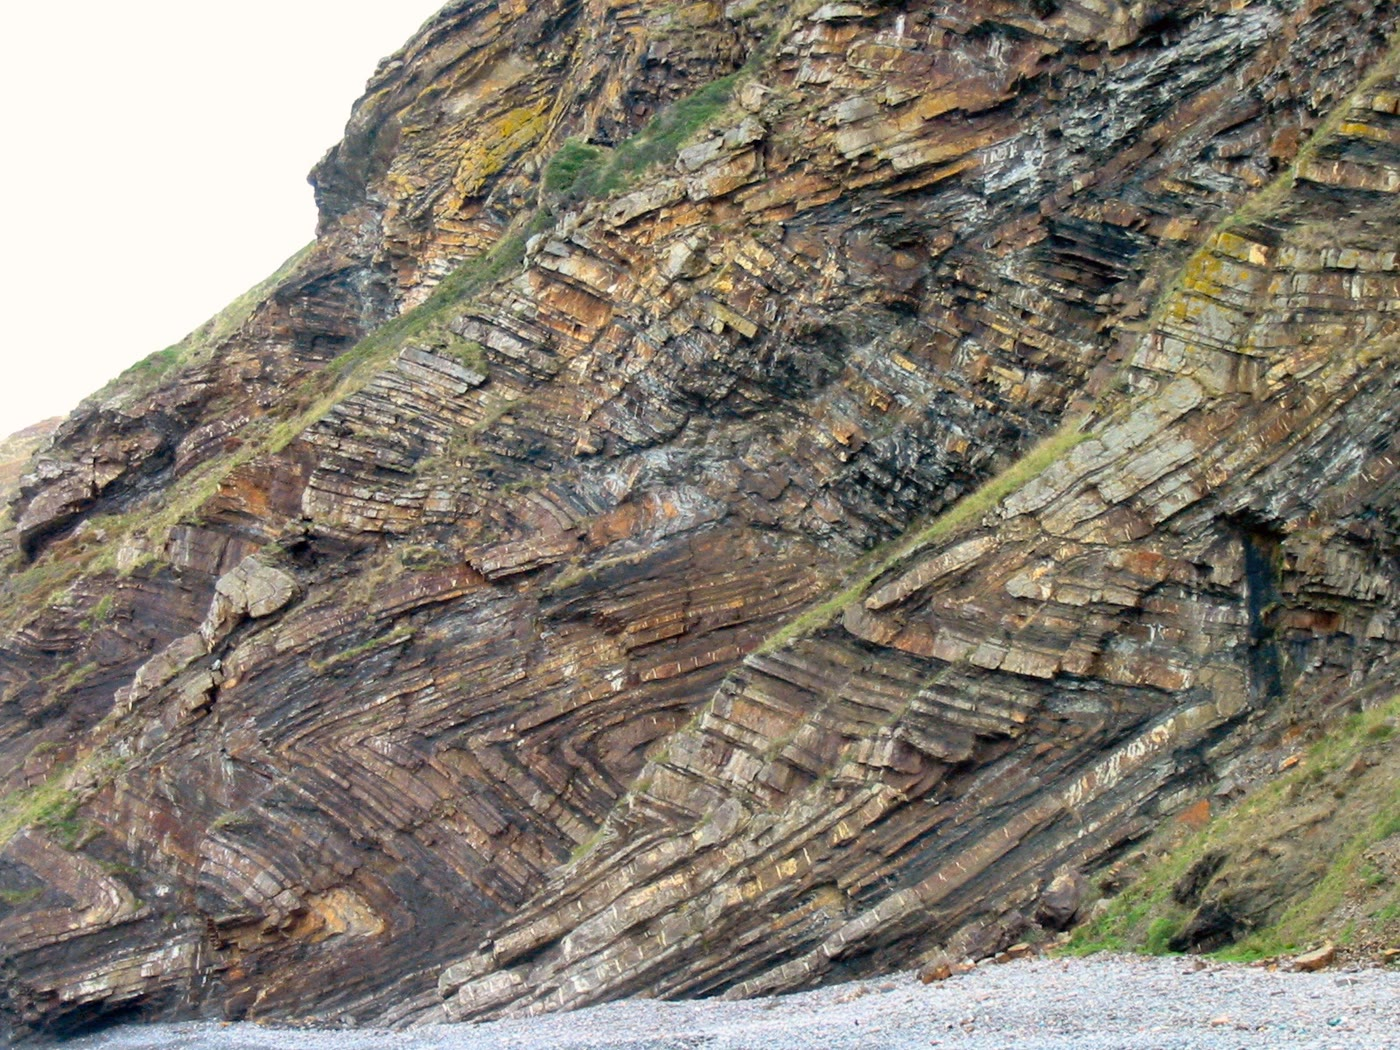
\includegraphics[width=0.78\linewidth]{images/book3/b1-chevron-folds-millook.jpg}
\par\smallskip{\small Bancs plissés de grès et de schiste dans les falaises de
Millook, au nord de la Cornouailles~: \omterm{def:b1:geological-maps:fold}{plis} en chevrons à \omterm{def:b1:faults-folds-fabrics:fold-elements}{flancs} presque droits et à \omterm{def:b1:faults-folds-fabrics:fold-elements}{charnières}
vives, leurs plans axiaux proches de la verticale. Photographie~: Smalljim, CC~BY~3.0
(Wikimedia Commons).}
\label{fig:b1:faults-folds-fabrics:chevrons}
\end{omfigure}
% ledger: commons:millook

\section{Les fabriques}\label{sec:b1:faults-folds-fabrics:fabrics}

Une roche déformée est souvent déformée dans toute sa masse, pas seulement sur quelques surfaces~: ses
grains sont aplatis, tournés ou recristallisés dans une orientation commune, ce qui lui
donne une fabrique. Une fabrique plane fait se débiter la roche, une fabrique linéaire la fait se briser
en bâtonnets.

\begin{definition}[Foliation, schistosité, clivage ardoisier, clivage de plan axial]\label{def:b1:faults-folds-fabrics:foliation}
Une \emph{foliation}\index{foliation} est une fabrique plane qui pénètre une roche~:
un ensemble de surfaces parallèles très rapprochées, faites de grains lamellaires ou aplatis alignés
ou de minces couches, le long desquelles la roche se débite le plus facilement.
La \emph{schistosité}\index{schistosite@schistosité} est la foliation d'un schiste, faite de
grains alignés plus gros qu'environ \qty{1}{mm}. Un \emph{clivage}\index{clivage (d'une roche)} est
une foliation d'une roche à grain fin faite par sa déformation~;
le \emph{clivage ardoisier}\index{clivage ardoisier} est le clivage d'une ardoise, fait
de silicates en feuillets trop petits pour être vus à l'œil nu, et si serrés
que la roche peut être fendue presque n'importe où en minces feuillets. Un
\emph{clivage de plan axial}\index{clivage de plan axial} est un clivage parallèle, ou presque parallèle, aux plans axiaux
des \omterm{def:b1:geological-maps:fold}{plis} des mêmes roches.
\end{definition}
% ledger: ws:fabrics

Une \omterm{def:b1:faults-folds-fabrics:foliation}{foliation} se forme à peu près perpendiculairement à la direction de plus grand
raccourcissement, par la rotation de grains lamellaires, la croissance de nouveaux \omterm{def:b1:rock-forming-minerals:groups}{micas}, et la
dissolution de grains sur les faces les plus pressées. Le \omterm{def:b1:faults-folds-fabrics:foliation}{clivage}
d'une ardoise n'a donc rien à voir avec la stratification de la boue~: il enregistre la
compression. Quand les \omterm{def:b1:geological-maps:fold}{plis} et le \omterm{def:b1:faults-folds-fabrics:foliation}{clivage} croissent dans le même raccourcissement, le \omterm{def:b1:faults-folds-fabrics:foliation}{clivage}
se trouve près des plans axiaux des \omterm{def:b1:geological-maps:fold}{plis}, et il s'ouvre légèrement en éventail à leur travers,
convergent ou divergent selon la résistance de chaque couche, comme le
montre la photographie ci-dessous.
% ledger: ws:fabrics

\begin{omfigure}
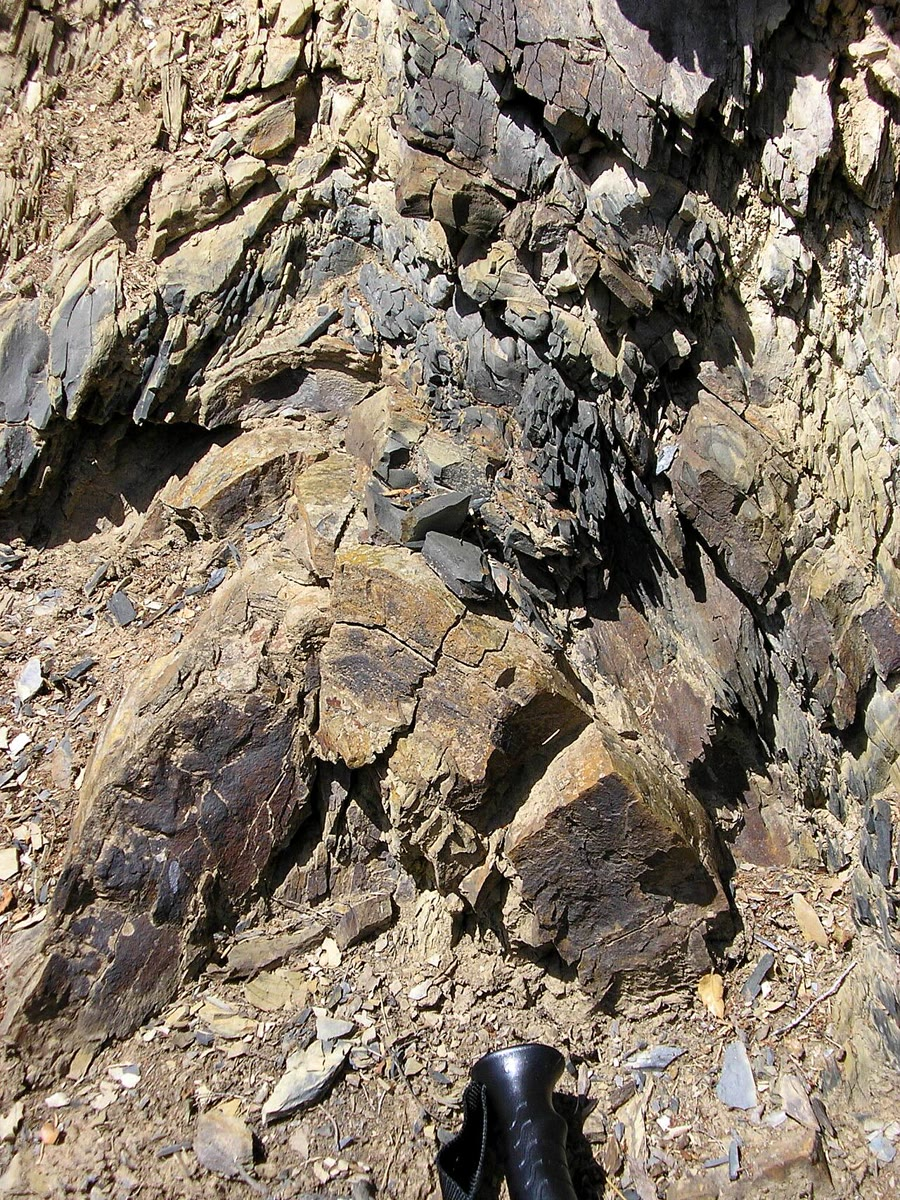
\includegraphics[height=8.2cm]{images/book3/b1-axial-planar-cleavage.jpg}
\par\smallskip{\small Un petit \omterm{def:b1:geological-maps:fold}{anticlinal} dans une alternance de grès et de schiste d'âge
carbonifère, près de Potes, en Cantabrie. Les bancs de grès bruns s'arquent au-dessus de
la \omterm{def:b1:faults-folds-fabrics:fold-elements}{charnière} au milieu du bas de l'image~; dans le schiste sombre au-dessus d'eux le
\omterm{def:b1:faults-folds-fabrics:foliation}{clivage}, un ensemble de fractures raides et très rapprochées recoupant les bancs, est
de \omterm{def:b1:faults-folds-fabrics:fold-elements}{plan axial}~: presque parallèle au \omterm{def:b1:faults-folds-fabrics:fold-elements}{plan axial} du \omterm{def:b1:geological-maps:fold}{pli}, il s'ouvre en éventail à
travers lui, l'éventail changeant d'une couche à l'autre. Le manche du bâton de marche fait environ \qty{4}{cm} de large.
Photographie~: Mikenorton, CC~BY-SA~3.0 (Wikimedia Commons).}
\label{fig:b1:faults-folds-fabrics:cleavage}
\end{omfigure}
% ledger: commons:axial-cleavage

\begin{definition}[Linéation, linéation d'intersection, linéation d'étirement]\label{def:b1:faults-folds-fabrics:lineation}
Une \emph{linéation}\index{lineation@linéation} est une fabrique linéaire qui pénètre une roche,
mesurée par sa direction et son \omterm{def:b1:field-lab-methods-1:trend-plunge}{plongement}. Une \emph{linéation
d'intersection}\index{lineation d'intersection@linéation d'intersection} est l'ensemble des droites selon lesquelles deux
fabriques planes se coupent, comme la stratification et un \omterm{def:b1:faults-folds-fabrics:foliation}{clivage}~; une
\emph{linéation d'étirement}\index{lineation d'etirement@linéation d'étirement} est faite de grains ou de
galets étirés selon la direction du plus grand étirement.
\end{definition}
% ledger: ws:fabrics

\begin{proposition}[La linéation d'intersection d'un pli]\label{prop:b1:faults-folds-fabrics:intersection}
Dans un \omterm{def:b1:faults-folds-fabrics:fold-elements}{pli cylindrique} avec un \omterm{def:b1:faults-folds-fabrics:foliation}{clivage de plan axial}, la \omterm{def:b1:faults-folds-fabrics:lineation}{linéation d'intersection}
de la stratification et du \omterm{def:b1:faults-folds-fabrics:foliation}{clivage} est parallèle à la \omterm{def:b1:faults-folds-fabrics:fold-elements}{ligne de charnière},
partout sur le \omterm{def:b1:geological-maps:fold}{pli}.
\end{proposition}

\begin{proof}
Chaque surface de stratification d'un \omterm{def:b1:faults-folds-fabrics:fold-elements}{pli cylindrique} contient la direction de son
axe. Le \omterm{def:b1:faults-folds-fabrics:fold-elements}{plan axial} contient les \omterm{def:b1:faults-folds-fabrics:fold-elements}{lignes de charnière}, qui sont parallèles à
l'axe, donc il contient aussi cette direction, de même que chaque plan de \omterm{def:b1:faults-folds-fabrics:foliation}{clivage}
parallèle à lui. Deux plans non parallèles qui contiennent tous deux la même
direction se rencontrent selon une droite de cette direction.
\end{proof}

La proposition est le chemin du géologue de terrain vers le \omterm{def:b1:field-lab-methods-1:trend-plunge}{plongement} d'un \omterm{def:b1:geological-maps:fold}{pli} trop grand
pour être vu en entier~: sur tout \omterm{def:b1:geological-maps:geological-map}{affleurement} de l'un ou l'autre flanc, les droites selon lesquelles le
\omterm{def:b1:faults-folds-fabrics:foliation}{clivage} coupe la stratification donnent la \omterm{def:b1:faults-folds-fabrics:fold-elements}{ligne de charnière}. La stratification et le \omterm{def:b1:faults-folds-fabrics:foliation}{clivage}
ensemble en disent plus~: où est le \omterm{def:b1:geological-maps:fold}{pli}, et de quel côté sont les bancs.

\begin{definition}[Vergence]\label{def:b1:faults-folds-fabrics:vergence}
La \emph{vergence}\index{vergence} d'un \omterm{def:b1:geological-maps:fold}{pli} asymétrique est la direction horizontale
vers laquelle sa partie supérieure s'est déplacée par rapport à sa partie inférieure~:
la direction dans laquelle il est renversé ou, pour un \omterm{def:b1:faults-folds-fabrics:fold-classes}{pli incliné}, vers laquelle
il penche.
\end{definition}
% ledger: ws:vergence

\begin{proposition}[Stratification et clivage sur les flancs d'un pli]\label{prop:b1:faults-folds-fabrics:cleavage-bedding}
Considérons un \omterm{def:b1:geological-maps:fold}{pli} à \omterm{def:b1:faults-folds-fabrics:fold-elements}{flancs} droits et à \omterm{def:b1:faults-folds-fabrics:foliation}{clivage de plan axial}, dans des roches
qui étaient à l'endroit avant le plissement, et dont les deux \omterm{def:b1:faults-folds-fabrics:fold-elements}{flancs} descendent
de chaque \omterm{def:b1:faults-folds-fabrics:fold-elements}{charnière} d'\omterm{def:b1:geological-maps:fold}{anticlinal}. Vu dans le profil~:
\begin{enumerate}[label=(\alph*)]
  \item sur un flanc où la stratification et le \omterm{def:b1:faults-folds-fabrics:foliation}{clivage} plongent dans le même sens, la
        stratification est la plus raide des deux exactement quand le flanc est
        renversé~;
  \item la rotation aiguë qui amène le \omterm{def:b1:faults-folds-fabrics:foliation}{clivage} sur la stratification a des
        sens opposés sur les deux \omterm{def:b1:faults-folds-fabrics:fold-elements}{flancs} d'un \omterm{def:b1:geological-maps:fold}{pli}~; sur un flanc non renversé,
        elle déplace le haut du \omterm{def:b1:faults-folds-fabrics:foliation}{clivage} horizontalement vers la \omterm{def:b1:faults-folds-fabrics:fold-elements}{charnière}
        d'\omterm{def:b1:geological-maps:fold}{anticlinal} au sommet de ce flanc.
\end{enumerate}
\end{proposition}

\begin{proof}
Regardons le long de la \omterm{def:b1:faults-folds-fabrics:fold-elements}{charnière} avec le \omterm{def:b1:faults-folds-fabrics:fold-elements}{plan axial} plongeant vers la gauche de l'angle
$\gamma$, $0 < \gamma \le \ang{90}$, et comptons les angles dans le sens antihoraire à partir de
l'horizontale pointant vers la droite. Le \omterm{def:b1:faults-folds-fabrics:foliation}{clivage}, parallèle au \omterm{def:b1:faults-folds-fabrics:fold-elements}{plan axial}, monte
à l'angle $\gamma$. À une \omterm{def:b1:faults-folds-fabrics:fold-elements}{charnière} d'\omterm{def:b1:geological-maps:fold}{anticlinal} les deux \omterm{def:b1:faults-folds-fabrics:fold-elements}{flancs} partent
vers le bas aux angles $\ang{180} + \gamma - \iota/2$ (flanc~1) et
$\ang{180} + \gamma + \iota/2$ (flanc~2), de part et d'autre du \omterm{def:b1:faults-folds-fabrics:fold-elements}{plan axial},
avec $\iota/2 \le \gamma$ puisque les deux descendent~; chaque flanc d'un train de \omterm{def:b1:geological-maps:fold}{plis}
est l'un de ces deux pour l'\omterm{def:b1:geological-maps:fold}{anticlinal} à son sommet. Les roches rajeunissent vers l'extérieur,
en s'éloignant du cœur de l'\omterm{def:b1:geological-maps:fold}{anticlinal}, le long de la normale au flanc qui pointe
loin du \omterm{def:b1:faults-folds-fabrics:fold-elements}{plan axial}.

Le flanc~1 descend vers la gauche~: il plonge vers la gauche de $\gamma - \iota/2$, moins
raide que le \omterm{def:b1:faults-folds-fabrics:foliation}{clivage}. Sa normale extérieure, à $\ang{90} + \gamma -
\iota/2$, pointe vers le haut~: il est à l'endroit. En montant, il fait
l'angle $\gamma - \iota/2$, donc la rotation aiguë du \omterm{def:b1:faults-folds-fabrics:foliation}{clivage} à la stratification
est horaire, de $\iota/2$~: le haut du \omterm{def:b1:faults-folds-fabrics:foliation}{clivage} se déplace vers la droite,
là où est la \omterm{def:b1:faults-folds-fabrics:fold-elements}{charnière}, puisque le flanc quitte la \omterm{def:b1:faults-folds-fabrics:fold-elements}{charnière} vers la gauche.

Le flanc~2 fait l'angle $\gamma + \iota/2$ avec l'horizontale, vers le haut. Si
$\gamma + \iota/2 > \ang{90}$, il descend vers la droite et plonge vers la
droite, à l'opposé du \omterm{def:b1:faults-folds-fabrics:foliation}{clivage}~; sa normale extérieure, à $\ang{270} + \gamma +
\iota/2$, a la composante vers le haut $-\cos(\gamma + \iota/2) > 0$~: il est à
l'endroit. Si $\gamma + \iota/2 < \ang{90}$, il descend vers la gauche,
plongeant vers la gauche de $\gamma + \iota/2$, plus raide que le \omterm{def:b1:faults-folds-fabrics:foliation}{clivage}, et
la même composante est négative~: le flanc est renversé. Dans les deux cas la rotation
aiguë du \omterm{def:b1:faults-folds-fabrics:foliation}{clivage} à la stratification est antihoraire, de $\iota/2$,
et déplace le haut du \omterm{def:b1:faults-folds-fabrics:foliation}{clivage} vers la gauche~; quand le flanc est à l'endroit
il quitte la \omterm{def:b1:faults-folds-fabrics:fold-elements}{charnière} vers la droite, donc la \omterm{def:b1:faults-folds-fabrics:fold-elements}{charnière} est à gauche. Les \omterm{def:b1:faults-folds-fabrics:fold-elements}{flancs}
qui plongent dans le même sens que le \omterm{def:b1:faults-folds-fabrics:foliation}{clivage} sont donc le flanc~1, moins raide, et un
flanc~2 renversé, plus raide, ce qui est (a)~; les sens sont horaire sur le flanc~1
et antihoraire sur le flanc~2, ce qui est (b).
\end{proof}

Le sens de la rotation change donc à chaque \omterm{def:b1:faults-folds-fabrics:fold-elements}{charnière}, \omterm{def:b1:geological-maps:fold}{anticlinal} ou \omterm{def:b1:geological-maps:fold}{synclinal}.
Un géologue qui l'enregistre le long d'un itinéraire trouve les \omterm{def:b1:faults-folds-fabrics:fold-elements}{charnières} de \omterm{def:b1:geological-maps:fold}{plis} trop
grands pour être vus sur un \omterm{def:b1:geological-maps:geological-map}{affleurement} là où le sens change, et les \omterm{def:b1:faults-folds-fabrics:fold-elements}{flancs} renversés
là où la stratification est plus raide que le \omterm{def:b1:faults-folds-fabrics:foliation}{clivage}~; le mot \omterm{def:b1:faults-folds-fabrics:vergence}{vergence} est aussi employé
pour ce sens de rotation, et les inversions de \omterm{def:b1:faults-folds-fabrics:vergence}{vergence} des \omterm{def:b1:geological-maps:fold}{plis} mineurs sont
cartographiées de la même façon pour trouver les \omterm{def:b1:faults-folds-fabrics:fold-elements}{charnières} des \omterm{def:b1:geological-maps:fold}{plis} majeurs~: les petits \omterm{def:b1:geological-maps:fold}{plis} sur
les deux \omterm{def:b1:faults-folds-fabrics:fold-elements}{flancs} d'un grand ont des asymétries opposées, et sa trace axiale
passe entre eux.
% ledger: ws:vergence, ws:fold-elements

\begin{omfigure}
\begin{tikzpicture}[>={Stealth[length=5pt]}, font=\small]
% a train of chevron folds seen along the hinge (north into the page, east to the right):
% axial planes dipping 60 deg to the west, interlimb angle 40 deg; long limbs dip 40 deg W
% (the right way up), short limbs 80 deg W (overturned). Short limb: from an anticline hinge H_k,
% length s along 260 deg to the syncline hinge S_k; long limb back up along 40 deg to H_{k+1},
% so that all anticline hinges are level, a wavelength w apart.
% Five bedding surfaces, repeated along the axial direction (similar folds); cleavage parallel to it.
\def\s{2.6}
\pgfmathsetmacro{\sx}{\s*cos(260)}\pgfmathsetmacro{\sy}{\s*sin(260)}
\pgfmathsetmacro{\w}{\sx - \sy/tan(40)}
\pgfmathsetmacro{\hx}{0.62*cos(60)}\pgfmathsetmacro{\hy}{0.62*sin(60)}
\newcommand{\surface}[1]{%
  (-\w+#1*\hx, #1*\hy) \foreach \k in {-1,0,1,2,3} { -- ({\k*\w+\sx+#1*\hx}, {\sy+#1*\hy}) -- ({(\k+1)*\w+#1*\hx}, {#1*\hy}) }}
\begin{scope}
  \clip (0.35,-3.3) rectangle (10.0,2.95);
  \begin{scope}
    \clip \surface{0} -- (12,6) -- (-4,6) -- cycle;
    \clip \surface{4} -- (12,-6) -- (-4,-6) -- cycle;
    \fill[omLithSand!45] (-4,-6) rectangle (12,6);
    \fill[omLithShale!40] \surface{2} -- (12,6) -- (-4,6) -- cycle;
    \fill[omLithSand!45] \surface{3} -- (12,6) -- (-4,6) -- cycle;
    \foreach \c in {-8.0,-7.78,...,13.0} {
      \draw[omDef!85, line width=0.35pt] ({\c-6*cot(60)},-6) -- ({\c+6*cot(60)},6);
    }
  \end{scope}
  \foreach \j in {0,1,2,3,4} { \draw[line width=0.75pt, line join=round] \surface{\j}; }
\end{scope}
% axial traces through the anticline hinges, and labels
\foreach \k in {1,2,3} {
  \draw[omThm, dashed, line width=0.6pt] ({\k*\w-0.5*cos(60)},{-0.5*sin(60)}) -- ({\k*\w+3.6*cos(60)},{3.6*sin(60)});
  \node[omThm, font=\scriptsize, anchor=south] at ({\k*\w+3.6*cos(60)},{3.6*sin(60)}) {anticlinal};
}
\foreach \k in {1,2,3} { \node[omThm, font=\scriptsize, anchor=north] at ({\k*\w+\sx},{\sy-0.15}) {synclinal}; }
\end{tikzpicture}
\par\smallskip{\small Un train de \omterm{def:b1:geological-maps:fold}{plis} en chevrons déversés vers la droite, en
profil, avec un \omterm{def:b1:faults-folds-fabrics:foliation}{clivage de plan axial} (fines lignes bleues), dessiné à l'échelle~: plans
axiaux plongeant de \ang{60} vers la gauche, \omterm{def:b1:faults-folds-fabrics:fold-elements}{angle entre flancs} \ang{40}. Les longs \omterm{def:b1:faults-folds-fabrics:fold-elements}{flancs}
plongent de \ang{40} vers la gauche, moins raide que le \omterm{def:b1:faults-folds-fabrics:foliation}{clivage}, et sont à
l'endroit~; les \omterm{def:b1:faults-folds-fabrics:fold-elements}{flancs} courts plongent de \ang{80} vers la gauche, plus raides que le
\omterm{def:b1:faults-folds-fabrics:foliation}{clivage}, et sont renversés. Amener le \omterm{def:b1:faults-folds-fabrics:foliation}{clivage} sur la stratification par
l'angle aigu est horaire sur chaque long flanc et antihoraire sur chaque
flanc court. Les \omterm{def:b1:geological-maps:fold}{plis} ont une \omterm{def:b1:faults-folds-fabrics:vergence}{vergence} vers la droite.}
\label{fig:b1:faults-folds-fabrics:vergence}
\end{omfigure}

\section{Les microstructures}\label{sec:b1:faults-folds-fabrics:micro}

Au microscope, la déformation d'une roche se lit dans ses grains. Un grain
de quartz courbé par le lent glissement de son réseau cristallin n'entre plus en
extinction d'un seul coup entre \omterm{def:b1:field-lab-methods-1:microscope}{polariseurs croisés}~: quand la platine tourne, une bande sombre
le balaie, parce que ses parties pointent dans des directions légèrement différentes.
Cette extinction ondulante (\cref{ch:b1:optical-mineralogy}) se renforce à mesure qu'on s'approche
d'une zone de cisaillement, parce que des défauts s'accumulent dans le réseau cristallin.
Là où l'eau est présente, les grains se dissolvent sur les faces où ils sont le plus pressés
et la matière dissoute se dépose là où la contrainte est plus faible, ou est
emportée~: cette dissolution par pression raccourcit les roches à basse température et
construit de nombreux \omterm{def:b1:faults-folds-fabrics:foliation}{clivages}. À plus haute température, les grains déformés sont
remplacés, tandis que la déformation se poursuit, par de nouveaux grains plus petits et non déformés,
d'abord le long des anciens joints de grains~: la recristallisation dynamique, qui réduit
la taille des grains et fait les \omterm{def:b1:faults-folds-fabrics:fault-rocks}{mylonites}. Les formes des grains déformés et des minéraux qui poussent dans
leur ombre montrent aussi dans quel sens une zone de cisaillement a joué~; ces indicateurs du sens de cisaillement,
et les mécanismes eux-mêmes, relèvent du volume de troisième année.
% ledger: ws:microstructures, ws:fabrics

\section{Exercices}

\begin{exercise}[$\star$]\label{exo:b1:faults-folds-fabrics:1}
Nommer chaque faille d'après le \omterm{def:b1:faults-folds-fabrics:fault-elements}{pitch} de son \omterm{def:b1:faults-folds-fabrics:fault-elements}{vecteur glissement}, le plan plongeant de \ang{60}~:
(a) $r = \ang{-90}$~; (b) $r = \ang{85}$~; (c) $r = 0$~; (d) $r = \ang{180}$~;
(e) $r = \ang{-40}$. (f) Comment (b) serait-elle appelée si son \omterm{def:b1:geological-maps:attitude}{pendage} était de \ang{25}~?
% ledger: ar:rake, usgs:fault-types
\end{exercise}

\begin{exercise}[$\star$]\label{exo:b1:faults-folds-fabrics:2}
Une \omterm{def:b1:faults-folds-fabrics:fault-types}{faille normale} plonge de \ang{55}~; son glissement est du pur glissement en \omterm{def:b1:geological-maps:attitude}{pendage}, avec un \omterm{def:b1:faults-folds-fabrics:fault-elements}{glissement net} de
\qty{300}{m}. Calculer son \omterm{def:b1:cross-sections:throw}{rejet vertical} et son \omterm{def:b1:cross-sections:throw}{rejet horizontal}.
\end{exercise}

\begin{exercise}[$\star$]\label{exo:b1:faults-folds-fabrics:3}
Donner l'\omterm{def:b1:faults-folds-fabrics:fold-elements}{angle entre flancs} et la classe de chaque \omterm{def:b1:faults-folds-fabrics:fold-classes}{pli droit}, dont les \omterm{def:b1:faults-folds-fabrics:fold-elements}{flancs} plongent
en sens opposés~: (a) \omterm{def:b1:faults-folds-fabrics:fold-elements}{flancs} plongeant de \ang{35} et \ang{35}~; (b) \ang{70}
et \ang{75}~; (c) \ang{85} et \ang{88}.
% ledger: ws:fold-classes
\end{exercise}

\begin{exercise}[$\star$]\label{exo:b1:faults-folds-fabrics:4}
Un grès a pour \omterm{def:b1:stress-strain-rheology:coulomb}{angle de frottement interne} \ang{35}. D'après la théorie d'Anderson,
sous quels angles plongent ses \omterm{def:b1:faults-folds-fabrics:fault-types}{failles normales} et ses \omterm{def:b1:faults-folds-fabrics:fault-types}{chevauchements}~? Quel
angle font entre elles deux \omterm{def:b1:faults-folds-fabrics:fault-types}{failles décrochantes} conjuguées~?
\end{exercise}

\begin{exercise}[$\star\star$]\label{exo:b1:faults-folds-fabrics:5}
Une faille a l'\omterm{def:b1:geological-maps:attitude}{attitude} $090/50$, et des \omterm{def:b1:faults-folds-fabrics:fault-rocks}{stries} de \omterm{def:b1:faults-folds-fabrics:fault-elements}{pitch} \ang{-30} sur elle~;
le \omterm{def:b1:faults-folds-fabrics:fault-elements}{glissement net} est de \qty{400}{m}. (a) Calculer les composantes en direction et en \omterm{def:b1:geological-maps:attitude}{pendage},
le \omterm{def:b1:cross-sections:throw}{rejet vertical} et le \omterm{def:b1:cross-sections:throw}{rejet horizontal}. (b) Écrire le \omterm{def:b1:faults-folds-fabrics:fault-elements}{vecteur glissement} en composantes est, nord
et haut, et donner sa direction et son \omterm{def:b1:field-lab-methods-1:trend-plunge}{plongement}. (c) Nommer la faille.
\end{exercise}

\begin{exercise}[$\star\star$]\label{exo:b1:faults-folds-fabrics:6}
Deux \omterm{def:b1:faults-folds-fabrics:fault-types}{failles décrochantes} verticales de même âge ont pour directions $020$ et $080$.
(a) D'après Anderson, donner les directions de $\sigma_1$, $\sigma_2$ et
$\sigma_3$, et l'\omterm{def:b1:stress-strain-rheology:coulomb}{angle de frottement interne} de la roche. (b) Laquelle des failles est
\omterm{def:b1:faults-folds-fabrics:fault-types}{dextre} et laquelle \omterm{def:b1:faults-folds-fabrics:fault-types}{senestre}~? Argumenter à partir du raccourcissement selon $\sigma_1$.
\end{exercise}

\begin{exercise}[$\star\star$]\label{exo:b1:faults-folds-fabrics:7}
Les deux \omterm{def:b1:faults-folds-fabrics:fold-elements}{flancs} d'un \omterm{def:b1:faults-folds-fabrics:fold-elements}{pli cylindrique} ont les \omterm{def:b1:geological-maps:attitude}{attitudes} $120/40$ et $260/30$.
Avec la \cref{prop:b1:faults-folds-fabrics:hinge}, trouver la direction et le \omterm{def:b1:field-lab-methods-1:trend-plunge}{plongement} de
sa \omterm{def:b1:faults-folds-fabrics:fold-elements}{ligne de charnière}, son \omterm{def:b1:faults-folds-fabrics:fold-elements}{angle entre flancs} et sa classe.
\end{exercise}

\begin{exercise}[$\star\star$]\label{exo:b1:faults-folds-fabrics:8}
Sur un \omterm{def:b1:geological-maps:geological-map}{affleurement}, la stratification a l'\omterm{def:b1:geological-maps:attitude}{attitude} $040/30$ et un \omterm{def:b1:faults-folds-fabrics:foliation}{clivage de plan axial}
l'\omterm{def:b1:geological-maps:attitude}{attitude} $160/80$. Trouver la direction et le \omterm{def:b1:field-lab-methods-1:trend-plunge}{plongement} de la \omterm{def:b1:faults-folds-fabrics:lineation}{linéation
d'intersection}. Que dit-elle du \omterm{def:b1:geological-maps:fold}{pli}~?
\end{exercise}

\begin{exercise}[$\star\star$]\label{exo:b1:faults-folds-fabrics:9}
Une faille verticale est de direction est--ouest. Un dyke vertical de direction nord--sud
la recoupe~; au nord de la faille le dyke se trouve \qty{350}{m} à l'est de là où
il est au sud de la faille. (a) La faille est-elle \omterm{def:b1:faults-folds-fabrics:fault-types}{dextre} ou \omterm{def:b1:faults-folds-fabrics:fault-types}{senestre}~? (b) Si les
\omterm{def:b1:faults-folds-fabrics:fault-rocks}{stries} sont horizontales, quel est le \omterm{def:b1:faults-folds-fabrics:fault-elements}{glissement net}~? (c) Si elles plongent au contraire de
\ang{20} vers l'est, quels sont le \omterm{def:b1:faults-folds-fabrics:fault-elements}{glissement net} et la composante verticale du
glissement, et quel bloc est descendu~?
\end{exercise}

\begin{exercise}[$\star\star\star$]\label{exo:b1:faults-folds-fabrics:10}
Une faille sans \omterm{def:b1:stress-strain-rheology:coulomb}{cohésion} et de coefficient de frottement $\mu$ fait l'angle
$\theta$ avec $\sigma_1$. (a) Montrer qu'elle glisse quand les \omterm{def:b1:stress-strain-rheology:principal}{contraintes principales} effectives
atteignent le rapport
\[
  \frac{\sigma_1'}{\sigma_3'} = \frac{1 + \mu\cot\theta}{1 - \mu\tan\theta} .
\]
(b) Avec $\mu = 0.6$ et $\sigma_1$ verticale, calculer le rapport pour des \omterm{def:b1:faults-folds-fabrics:fault-types}{failles normales}
plongeant de \ang{60}, \ang{45} et \ang{35}. (c) Montrer qu'une \omterm{def:b1:faults-folds-fabrics:fault-types}{faille normale}
plongeant de moins d'un certain angle ne peut jamais glisser, et calculer cet angle.
(d) Pour $\mu = 0.6$ et $\mu = 0.85$, donner les \omterm{def:b1:geological-maps:attitude}{pendages} des \omterm{def:b1:faults-folds-fabrics:fault-types}{failles normales} et
des \omterm{def:b1:faults-folds-fabrics:fault-types}{chevauchements} les mieux orientés.
\end{exercise}

\begin{exercise}[$\star\star\star$]\label{exo:b1:faults-folds-fabrics:11}
Le long d'un itinéraire est--ouest à travers des \omterm{def:b1:geological-maps:fold}{plis} en chevrons dont les \omterm{def:b1:faults-folds-fabrics:fold-elements}{charnières} sont orientées nord,
un \omterm{def:b1:faults-folds-fabrics:foliation}{clivage de plan axial} plonge de \ang{60} vers l'ouest partout. La stratification
plonge de \ang{40}~O à la station A, de \ang{80}~O à la station B et de \ang{40}~O à
la station C, de l'ouest vers l'est, dans des roches qui étaient à l'endroit avant
le plissement. (a) Quelle station est sur un flanc renversé~? (b) Dans quel sens
le \omterm{def:b1:faults-folds-fabrics:foliation}{clivage} tourne-t-il sur la stratification à chaque station, vu en regardant vers le nord~?
(c) Où sont les \omterm{def:b1:faults-folds-fabrics:fold-elements}{charnières}, et lesquelles sont des anticlinaux~? (d) Trouver l'\omterm{def:b1:faults-folds-fabrics:fold-elements}{angle entre flancs}
et l'\omterm{def:b1:geological-maps:attitude}{attitude} des plans axiaux, et dire vers où les \omterm{def:b1:geological-maps:fold}{plis}
ont leur \omterm{def:b1:faults-folds-fabrics:vergence}{vergence}.
\end{exercise}

\begin{exercise}[$\star\star\star$]\label{exo:b1:faults-folds-fabrics:12}
Une couche de longueur $L_0$ est plissée en un train de \omterm{def:b1:geological-maps:fold}{plis} en chevrons symétriques
d'\omterm{def:b1:faults-folds-fabrics:fold-elements}{angle entre flancs} $\iota$, sa longueur étant inchangée. (a) Montrer que sa longueur
mesurée à travers les \omterm{def:b1:geological-maps:fold}{plis} devient $L_0\sin(\iota/2)$. (b) Quel raccourcissement
représentent des \omterm{def:b1:geological-maps:fold}{plis} en chevrons d'\omterm{def:b1:faults-folds-fabrics:fold-elements}{angle entre flancs} \ang{60}~? (c) Quel \omterm{def:b1:faults-folds-fabrics:fold-elements}{angle entre flancs}
correspond à un raccourcissement de \qty{30}{\percent}~? (d) Un train de \omterm{def:b1:faults-folds-fabrics:fold-classes}{plis droits}
à \omterm{def:b1:faults-folds-fabrics:fold-elements}{flancs} plongeant de \ang{12}~: quel raccourcissement~?
\end{exercise}

\section{Problème~: Les structures des collines de Varden, mesurées}

\begin{problem}[{Problème du week-end --- l'anticlinal et la faille normale des
collines de Varden, des attitudes de leurs plans jusqu'au glissement sur la
faille}]
\label{pb:b1:faults-folds-fabrics:1}
% values: calc/ch17.py; region: figdata/shared/region.py (limbs, plunge, fault)
Les collines de Varden sont plissées en un \omterm{def:b1:geological-maps:fold}{anticlinal}, dont l'axe est nord--sud
en $x = \qty{3.5}{km}$, et un \omterm{def:b1:geological-maps:fold}{synclinal} à \qty{4}{km} à l'est de lui~; les deux
ont des \omterm{def:b1:faults-folds-fabrics:fold-elements}{flancs} plans. Un levé de terrain a mesuré la stratification sur le flanc est de
l'\omterm{def:b1:geological-maps:fold}{anticlinal} à $080.7/12.2$ et sur son flanc ouest à $279.3/12.2$. La couverture
est recoupée par une \omterm{def:b1:faults-folds-fabrics:fault-types}{faille normale} d'\omterm{def:b1:geological-maps:attitude}{attitude} $120/60$, dont le \omterm{def:b1:faults-folds-fabrics:fault-elements}{compartiment supérieur} s'est abaissé
le long du \omterm{def:b1:geological-maps:attitude}{pendage}, avec un \omterm{def:b1:cross-sections:throw}{rejet vertical} de \qty{200}{m}. Donner les angles à \ang{0.1} et les longueurs à
\qty{0.1}{m}.

\medskip
\noindent\textbf{Partie I --- Les flancs.}
\begin{enumerate}
  \item Écrire les normales unitaires vers le haut $\mathbf n_1$ (flanc est) et
        $\mathbf n_2$ (flanc ouest) en composantes est, nord et haut.
  \item Calculer $\mathbf n_1\cdot\mathbf n_2$ et l'angle entre les
        normales.
  \item En déduire l'\omterm{def:b1:faults-folds-fabrics:fold-elements}{angle entre flancs} de l'\omterm{def:b1:geological-maps:fold}{anticlinal}.
  \item Classer l'\omterm{def:b1:geological-maps:fold}{anticlinal} par son \omterm{def:b1:faults-folds-fabrics:fold-elements}{angle entre flancs}.
  \item Les deux \omterm{def:b1:faults-folds-fabrics:fold-elements}{flancs} plongent de \ang{12.2}. Pourquoi l'\omterm{def:b1:faults-folds-fabrics:fold-elements}{angle entre flancs} n'est-il pas exactement
        $\ang{180} - 2\times\ang{12.2}$~? Calculer le \omterm{def:b1:cross-sections:apparent-dip}{pendage apparent} de l'un ou l'autre
        flanc dans une coupe verticale est--ouest.
  \item Le \omterm{def:b1:geological-maps:fold}{synclinal} partage le flanc est de l'\omterm{def:b1:geological-maps:fold}{anticlinal}, et son propre flanc est
        est parallèle au flanc ouest de l'\omterm{def:b1:geological-maps:fold}{anticlinal}. Quel est son \omterm{def:b1:faults-folds-fabrics:fold-elements}{angle entre
        flancs}~?
\end{enumerate}

\medskip
\noindent\textbf{Partie II --- La ligne de charnière et le plan axial.}
\begin{enumerate}[resume]
  \item Calculer $\mathbf n_1\times\mathbf n_2$, et la direction et le \omterm{def:b1:field-lab-methods-1:trend-plunge}{plongement} de
        la \omterm{def:b1:faults-folds-fabrics:fold-elements}{ligne de charnière}.
  \item Donner l'\omterm{def:b1:geological-maps:attitude}{attitude} du \omterm{def:b1:faults-folds-fabrics:fold-elements}{plan axial}. L'\omterm{def:b1:geological-maps:fold}{anticlinal} est-il droit,
        incliné ou couché~?
  \item Donner la description complète du \omterm{def:b1:geological-maps:fold}{pli}~: serrage, \omterm{def:b1:geological-maps:attitude}{attitude} du
        \omterm{def:b1:faults-folds-fabrics:fold-elements}{plan axial}, \omterm{def:b1:field-lab-methods-1:trend-plunge}{plongement}.
  \item Sur la \omterm{def:b1:geological-maps:geological-map}{carte géologique} du \cref{ch:b1:geological-maps}, dans quel sens
        les \omterm{def:b1:geological-maps:geological-map}{affleurements} de l'\omterm{def:b1:geological-maps:fold}{anticlinal} se ferment-ils, et qu'est-ce qui affleure en son cœur~?
  \item Le schiste de la couverture porte un \omterm{def:b1:faults-folds-fabrics:foliation}{clivage de plan axial}. Donner son
        \omterm{def:b1:geological-maps:attitude}{attitude}, et la direction et le \omterm{def:b1:field-lab-methods-1:trend-plunge}{plongement} de sa \omterm{def:b1:faults-folds-fabrics:lineation}{linéation d'intersection} sur
        le flanc est.
  \item Sur le flanc est, dans quel sens le \omterm{def:b1:faults-folds-fabrics:foliation}{clivage} tourne-t-il sur la
        stratification, vu en regardant vers le nord, et de quel côté est la \omterm{def:b1:faults-folds-fabrics:fold-elements}{charnière} de l'\omterm{def:b1:geological-maps:fold}{anticlinal}~?
\end{enumerate}

\medskip
\noindent\textbf{Partie III --- La faille et les contraintes.}
\begin{enumerate}[resume]
  \item Donner la direction de la faille par la règle de la main droite, et dire de quel
        côté de sa trace se trouve le \omterm{def:b1:faults-folds-fabrics:fault-elements}{compartiment supérieur}.
  \item Quelle contrainte principale était verticale quand la faille s'est formée, d'après
        Anderson~?
  \item Donner les directions des deux \omterm{def:b1:stress-strain-rheology:principal}{contraintes principales} horizontales.
  \item Quel \omterm{def:b1:stress-strain-rheology:coulomb}{angle de frottement interne} le \omterm{def:b1:geological-maps:attitude}{pendage} implique-t-il~? Quel \omterm{def:b1:stress-strain-rheology:coulomb}{coefficient
        de frottement interne}~?
  \item Donner l'\omterm{def:b1:geological-maps:attitude}{attitude} de la famille conjuguée de failles que les mêmes
        contraintes auraient pu faire, et l'angle entre les deux familles.
  \item La faille serait-elle la mieux orientée pour glisser de nouveau dans le même régime,
        avec le frottement de Byerlee de 0.85~?
\end{enumerate}

\medskip
\noindent\textbf{Partie IV --- Le glissement.}
\begin{enumerate}[resume]
  \item Donner le \omterm{def:b1:faults-folds-fabrics:fault-elements}{pitch} du \omterm{def:b1:faults-folds-fabrics:fault-elements}{vecteur glissement}, et sa direction et son \omterm{def:b1:field-lab-methods-1:trend-plunge}{plongement}.
  \item Écrire le vecteur unitaire du glissement en composantes est, nord et haut.
  \item Calculer le \omterm{def:b1:cross-sections:throw}{rejet horizontal} de la faille.
  \item Calculer les composantes est et nord du déplacement horizontal
        du \omterm{def:b1:faults-folds-fabrics:fault-elements}{compartiment supérieur}.
  \item Vérifier que le \omterm{def:b1:faults-folds-fabrics:fault-elements}{glissement net} $L$, le \omterm{def:b1:cross-sections:throw}{rejet vertical} $h$ et le \omterm{def:b1:cross-sections:throw}{rejet horizontal} $e$ satisfont
        $L^2 = h^2 + e^2$, et expliquer pourquoi.
  \item Au mètre près, quel est le \omterm{def:b1:faults-folds-fabrics:fault-elements}{glissement net} sur la faille de Varden~?
\end{enumerate}
\end{problem}
